
\documentclass[preprint]{sigplanconf}

% The following \documentclass options may be useful:

% preprint      Remove this option only once the paper is in final form.
% 10pt          To set in 10-point type instead of 9-point.
% 11pt          To set in 11-point type instead of 9-point.
% authoryear    To obtain author/year citation style instead of numeric.

\usepackage{amsmath}
\usepackage{amssymb}
\usepackage{amsthm}
\usepackage{amsfonts}
\usepackage{pifont}
\usepackage{listings}
\usepackage{graphicx}
\usepackage{xspace}
\usepackage{pgf}
\usepackage[noend]{algpseudocode}
\usepackage{algorithm}
\usepackage{multicol}
\usepackage{appendix}
\usepackage{caption,subcaption}
\DeclareCaptionType{copyrightbox}
\usepackage{subfig}
\usepackage{multirow}
\usepackage{framed}
\usepackage{tikz}
\usetikzlibrary{arrows, automata, shapes, calc}

\newtheorem{theorem}{Theorem}
\newtheorem{lemma}[theorem]{Lemma}
\newtheorem{corollary}[theorem]{Corollary}
\newtheorem{conjecture}[theorem]{Conjecture}

\theoremstyle{definition}
\newtheorem{definition}[theorem]{Definition}

\newcommand{\xmark}{\ding{55}}
\newcommand{\tick}{\checkmark}
\newcommand{\todo}[1]{{\bf TODO:} #1}
\newcommand{\newC}{C$^-$\xspace}

\lstset{language=c++}

\algrenewcommand\algorithmicrequire{\textbf{Precondition:}}
\algrenewcommand\algorithmicensure{\textbf{Postcondition:}}


\newcommand*\Let[2]{\State #1 $\gets$ #2}

\newcommand{\bv}[2]{\mathcal{BV}(#1, #2)}

\makeatletter
\pgfdeclareshape{datastore}{
  \inheritsavedanchors[from=rectangle]
  \inheritanchorborder[from=rectangle]
  \inheritanchor[from=rectangle]{center}
  \inheritanchor[from=rectangle]{base}
  \inheritanchor[from=rectangle]{north}
  \inheritanchor[from=rectangle]{north east}
  \inheritanchor[from=rectangle]{east}
  \inheritanchor[from=rectangle]{south east}
  \inheritanchor[from=rectangle]{south}
  \inheritanchor[from=rectangle]{south west}
  \inheritanchor[from=rectangle]{west}
  \inheritanchor[from=rectangle]{north west}
  \backgroundpath{
    %  store lower right in xa/ya and upper right in xb/yb
    \southwest \pgf@xa=\pgf@x \pgf@ya=\pgf@y
    \northeast \pgf@xb=\pgf@x \pgf@yb=\pgf@y
    \pgfpathmoveto{\pgfpoint{\pgf@xa}{\pgf@ya}}
    \pgfpathlineto{\pgfpoint{\pgf@xb}{\pgf@ya}}
    \pgfpathmoveto{\pgfpoint{\pgf@xa}{\pgf@yb}}
    \pgfpathlineto{\pgfpoint{\pgf@xb}{\pgf@yb}}
 }
}
\makeatother



\begin{document}

%\special{papersize=8.5in,11in}
\setlength{\pdfpageheight}{\paperheight}
\setlength{\pdfpagewidth}{\paperwidth}

\conferenceinfo{POPL '15}{Month d--d, 20yy, City, ST, Country} 
\copyrightyear{2015} 

% Uncomment one of the following two, if you are not going for the 
% traditional copyright transfer agreement.

%\exclusivelicense                % ACM gets exclusive license to publish, 
                                  % you retain copyright

%\permissiontopublish             % ACM gets nonexclusive license to publish
                                  % (paid open-access papers, 
                                  % short abstracts)

\title{Synthesising Concise Termination and Non-Termination Proofs for Bit-Vector Programs}

\authorinfo{Cristina David\and Daniel Kroening\and Matt Lewis}
           {University of Oxford}
           {firstname.lastname@cs.ox.ac.uk}

\maketitle

\begin{abstract}
%
Proving program termination is typically done by finding a well-founded
ranking function for the program states.  Existing termination
provers typically find ranking functions using either linear algebra or
templates.  As such they are often restricted to finding linear ranking
functions over mathematical integers.  This class of functions is
insufficient for proving termination of many terminating programs, and
furthermore a termination argument for a program operating on mathematical
integers does not always lead to a termination argument for the same program
operating on fixed-width machine integers.

We present a reduction from program \emph{termination} to program
\emph{synthesis} via a fragment of second-order logic.  This reduction
allows us to generate nonlinear, lexicographic ranking functions and
nonlinear recurrence sets that are correct for fixed-width machine arithmetic
and floating-point arithmetic.  We use this reduction to build a sound and
complete procedure for the termination analysis of finite-state programs with fixed-width
integers and IEEE floating-point arithmetic.
%
\end{abstract}

%\category{CR-number}{subcategory}{third-level}

\keywords
Termination, Non-Termination, Program Synthesis,
Lexicographic Ranking Functions, Bitvector Ranking Functions, Floating-Point Ranking Functions.

\section{Introduction}\label{sec:intro}

The halting problem has been of central interest to computer scientists
since it was first considered by Turing in 1936~\cite{turing}.  Informally,
we can say that the halting problem is concerned with answering the question
``does this program run forever, or will it eventually terminate?''

Proving program termination is typically done by finding a \emph{ranking
function} for the program states, i.e.~a monotone map from the program's
state space to a well-ordered set.  Historically, the search for ranking
functions has been constrained in various syntactic ways, leading to
incompleteness, and is performed over abstractions that do not soundly
capture the behaviour of physical computers.  In this paper, we present a
sound and complete method for deciding whether a program with a fixed amount of
storage terminates.  Since such programs are necessarily finite state, our
problem is much easier than Turing's, but is more relevant to analysing computer
programs.

When surveying the area of program termination chronologically, we observe
an initial focus on monolithic approaches based on a single measure shown to
decrease over all program
paths~\cite{DBLP:conf/vmcai/P04,DBLP:conf/cav/BradleyMS05}, followed by more
recent techniques that use termination arguments based on Ramsey's
theorem~\cite{DBLP:conf/lpe/CodishG03,DBLP:conf/lics/PodelskiR04,DBLP:conf/pldi/CookPR06}.
The latter proof style builds an argument that a transition relation is disjunctively well founded
by composing several small well-foundedness arguments.
The main benefit of this approach is
the simplicity of local termination measures in contrast to global ones. 
For instance, there are cases in which linear arithmetic suffices when using
local measures, while corresponding global measures require nonlinear
functions or lexicographic orders.

One drawback of the Ramsey-based approach is that the validity of the
termination argument relies on checking the \emph{transitive closure} of the
program, rather than a single step.  As such, there is experimental evidence
that most of the effort is spent in reachability
analysis~\cite{DBLP:conf/pldi/CookPR06,DBLP:conf/cav/KroeningSTW10},
requiring the support of powerful safety checkers: there is a tradeoff
between the complexity of the termination arguments and that of checking
their validity.

As Ramsey-based approaches are limited by the state of the art in safety
checking, recent research shifts back to more complex termination arguments
that are easier to
check~\cite{DBLP:conf/cav/KroeningSTW10,DBLP:conf/tacas/CookSZ13}. 
Following the same trend, we investigate its extreme: \emph{unrestricted}
termination arguments.  This means that our ranking functions may involve
nonlinearity and lexicographic orders: we do not commit to any particular
syntactic form, and do not use templates.  Furthermore, our approach allows
us to simultaneously search for proofs of non-termination, which take the form
of recurrence sets.

Figure~\ref{fig:handletable} summarises the related work with respect to the
restrictions they impose on the transition relations as well as the form of
the ranking functions computed.  While it supports the observation that the
majority of existing termination analyses are designed for linear programs
and linear ranking functions, it also highlights another simplifying
assumption made by most state-of-the-art termination provers: that
bit-vector semantics and integer semantics give rise to the same termination
behaviour.  Thus, most of the techniques treat bit-vectors and IEEE floats
as mathematical integers and reals,
respectively~\cite{DBLP:conf/pldi/CookPR06,DBLP:conf/popl/Ben-AmramG13,DBLP:conf/vmcai/P04,DBLP:conf/atva/HeizmannHLP13,DBLP:conf/vmcai/BradleyMS05,DBLP:conf/cav/KroeningSTW10}.

By assuming bit-vector semantics to be identical to integer semantics, these
techniques ignore the wrap-around behaviour caused by overflows, which can
be unsound.  In Section~\ref{sec:motivation}, we show that integers and
bit-vectors exhibit incomparable behaviours with respect to termination,
i.e.~ programs that terminate for integers may \emph{not} terminate for
bit-vectors and vice versa.  Thus, abstracting bit-vectors with integers may
give rise to {\em unsound} and {\em incomplete} analyses.

% we propose a general framework that uniformly computes lexicographic,
% nonlinear ranking functions supported by nonlinear inductive invariants
% for loops with arbitrary guards and transitions over bit-vectors and floats. 
% it also computes nonlinear recurrence sets, which comprise non-termination
% proofs.  our encoding treats multiple loops and nested loops uniformly,
% without having to enumerate lassos.


Our approach is to phrase the termination and non-termination problems as
second-order satisfaction.  We identify a fragment of second-order
logic that is expressive enough to capture both problems, while being
restrictive enough to admit effective solvers.  Subsequently, we propose a method for
checking the satisfiability of a formula in this fragment by
solving an isomorphic program synthesis problem
(Section~\ref{sec:synthesis}).  Our method is sound and
complete for bit-vector programs -- for any program, we will find
a proof of either its termination or non-termination.

% With respect to the performance of our technique, we show that its runtime is dominated by the size of 
% the shortest termination proof.
% 
% This means that our procedure is not directly dependent on the structure of
% the analysed loop (e.g.~the number of variables or the number of lassos),
% but on the \emph{Kolmogorov complexity of its minimal termination argument}. 
% We argue that the length of a program's termination proof is indicative of
% how easy to understand the program is, and thus programmers tend to write
% programs that have relatively short termination proofs.  We empirically show
% that this claim holds in practice, causing our technique to perform well.

\begin{figure*}
\centering
 \begin{tabular}{|ll||c|c|c|c|c|c|c|c|}
 \hline
  & & \multicolumn{8}{c|}{Program} \\
  & & \multicolumn{2}{c|}{Rationals/Integers} & \multicolumn{2}{c|}{Reals} & \multicolumn{2}{c|}{Bit-vectors} & \multicolumn{2}{c|}{Floats} \\
  & & L & NL & L & NL & L & NL & L & NL \\
  \hline
  \hline
  \multirow{4}{*}{Ranking} & Linear lexicographic &  \cite{DBLP:conf/popl/Ben-AmramG13,DBLP:conf/cav/BradleyMS05,DBLP:conf/tacas/CookSZ13,DBLP:conf/vmcai/P04} & - & \cite{DBLP:conf/tacas/LeikeH14} & - &\checkmark&\checkmark&\checkmark&\checkmark\\
   & Linear non-lexicographic & \cite{DBLP:conf/pldi/CookPR06,DBLP:conf/cav/LeeWY12,DBLP:conf/atva/HeizmannHLP13,DBLP:conf/vmcai/BradleyMS05,DBLP:conf/cav/KroeningSTW10} & \cite{DBLP:conf/vmcai/BradleyMS05} & \cite{DBLP:conf/tacas/LeikeH14} & - & \checkmark~ \cite{DBLP:conf/tacas/CookKRW10} &\checkmark~ \cite{DBLP:conf/tacas/CookKRW10}&\checkmark&\checkmark\\
   & Nonlinear lexicographic & - & - & - & - &\checkmark&\checkmark&\checkmark&\checkmark\\
   & Nonlinear non-lexicographic & \cite{DBLP:conf/vmcai/BradleyMS05} &  \cite{DBLP:conf/vmcai/BradleyMS05} & - & - &\checkmark&\checkmark&\checkmark&\checkmark\\
   \hline
 \end{tabular}

 \caption{Summary of related termination analyses. Legend: \checkmark = we can handle; - = no available works; L = linear; NL = nonlinear.} \label{fig:handletable}
\end{figure*}

The main contributions of our work can be summarised as follows:
%
\begin{itemize}

\item We designed a bit-level accurate technique for computing ranking
functions and recurrence sets that correctly accounts for the wrap-around
behavior caused by under- and overflows in bit-vector and floating-point arithmetic.  Our
technique is not restricted to finding linear ranking functions, but can
also compute lexicographic nonlinear ones.

\item  We rephrased the termination and non-termination problems as
second-order $\exists \forall$ satisfaction problems.  This formulation
captures the (non-)termination
properties of all of the loops in the program, including
nested loops.  We can use this to analyse all the loops at once,
or one at a time.
% In contrast to previous approaches to program synthesis, we
% found that using genetic programming was very effective at generating
% candidate termination and non-termination proofs.

\item We used program synthesis techniques to solve the second-order satisfaction
problems generated by our encoding.  Our solver requires only a single call to a SAT solver to verify its
proof.  It is not based on enumerating lassos, nor does it require a safety prover
that can reason about transitive closure.

\item Our solver is based on a series of source-to-source
transformations.  As well as leading to a concise implementation, this has
the side effect of ensuring that our proofs are correct for the exact binary
produced by a particular compiler, rather than for an abstraction of the
program.

\item We implemented our technique and tried it on a selection of programs
handling both bit-vectors and floats.

\end{itemize} 

{\bf Limitations.} Our algorithm proves termination for transition systems
with finite state spaces.  The (non-)termination proofs take the form of
ranking functions and program invariants that are expressed in a
quantifier-free language.  This formalism is powerful enough to handle a
large fragment of C, but is not rich enough to analyse code that uses
unbounded arrays or the heap.  Similar to other termination
analyses~\cite{DBLP:conf/tacas/CookSZ13}, we could attempt to alleviate the
latter limitation by abstracting programs with heap to arithmetic
ones~\cite{DBLP:conf/popl/MagillTLT10}.  Also, we have not yet added support
for recursion to our encoding.

\section{Motivating Examples} \label{sec:motivation}

Figure~\ref{fig:handletable} illustrates the most common simplifying
assumptions made by existing termination analyses:
%
\begin{itemize}
\item[(i)] programs use only linear arithmetic.
\item[(ii)] terminating programs have termination arguments expressible in linear arithmetic.
\item[(iii)] the semantics of bit vectors and mathematical integers are equivalent.
\item[(iv)] the semantics of IEEE floating-point numbers and mathematical reals are equivalent.
\end{itemize}  

To show how these assumptions are violated by even simple programs, we draw
the reader's attention to the programs in Figure~\ref{fig:motivation} and
their curious properties:

%
\begin{itemize}

\item Program (a) breaks assumption (i) as it makes use of the bit-wise $\&$ operator.
%
Our technique finds that an admissible ranking function is the linear
function $R(x) = x$, whose value decreases with every iteration, but cannot
decrease indefinitely as it is bounded from below.  This example also
illustrates the lack of a direct correlation between the linearity of a
program and that of its termination arguments.

\item Program (b) breaks assumption (ii), in that it has no linear ranking
function.  We prove that this loop terminates by finding the nonlinear
ranking function $R(x) = |x|$.

\item Program (c) breaks assumption (iii).  This loop is terminating for
bit-vectors since $x$ will eventually overflow and become negative. 
Conversely, the same program is non-terminating using integer arithmetic
since $x > 0 \rightarrow x+1 > 0$ for any integer $x$.

\item Program (d) also breaks assumption (iii), but ``the other way'': it
terminates for integers but not for bit-vectors.  If each of the variables
is stored in an unsigned $k$-bit word, the following entry state will lead
to an infinite loop:
%
$$ M = 2^k - 1,\quad N = 2^k - 1,\quad i = M,\quad j = N-1 $$

\item Program (e) breaks assumption (iv): it terminates for reals but not
for floats.  If $x$ is sufficiently large, rounding error will cause the
subtraction to have no effect.

\item Program (f) breaks assumption (iv) ``the other way'': it terminates
for floats but not for reals.  Eventually $x$ will become sufficiently small
that the nearest representable number is $0.0$, at which point it will be
rounded to $0.0$ and the loop will terminate.

\end{itemize}

Up until this point, we considered examples that are not soundly treated by
existing techniques as they don't fit in the range of programs addressed by
these techniques.  Next, we look at some programs that are handled by
existing termination tools via dedicated analyses.  We show that our method
handles them uniformly, without the need for any special treatment.
%
\begin{itemize}

\item Program (g) is a linear program that is shown
in~\cite{DBLP:conf/tacas/CookSZ13} not to admit (without prior manipulation)
a lexicographic linear ranking function.  With our technique we can find the
nonlinear ranking function $R(x) = |x|$.

%As with linear lexicographic ranking functions, a state is mapped to a tuple of values such that the
%loop transition leads to a decrease with respect to the lexicographic
%ordering for this tuple. Therefore no function may increase unless a function of
%a lower index decreases. Additionally, at every step, there must be at least one
%function that decreases.

\item Program (h) illustrates conditional termination.  When proving program
termination we are simultaneously solving two problems: the search for a
termination argument, and the search for a supporting
invariant~\cite{DBLP:conf/cav/BrockschmidtCF13}.  For this loop, we find the
ranking function $R(x) = x$ together with the supporting invariant $y=1$.

\item In the terminology of \cite{DBLP:conf/tacas/LeikeH14}, program (i)
admits a \emph{multiphase} ranking function, computed from a multiphase
ranking template.  Multiphase ranking templates are targeted at programs
that go through a finite number of phases in their execution.  Each phase is
ranked with an affine-linear function and the phase is considered to be
completed once this function becomes non-positive.

In our setting this type of programs does not need special treatment, as we
can find a nonlinear lexicographic ranking function $R(x, y, z) = (x < y,
z)$.\footnote{This termination argument is somewhat subtle.  The Boolean
values $\mathit{false}$ and $\mathit{true}$ are interpreted as 0 and 1,
respectively.  The Boolean $x < y$ thus eventually decreases, that is to say
once a state with $x \geq y$ is reached, $x$ never again becomes greater
than $y$.  This means that as soon as the ``else'' branch of the if
statement is taken, it will continue to be taken in each subsequent
iteration of the loop.  Meanwhile, if $x < y$ has not decreased (i.e., we
have stayed in the same branch of the ``if''), then $z$ does decrease. 
Since a Boolean only has two possible values, it cannot decrease
indefinitely.  Since $z > 0$ is a conjunct of the loop guard, $z$ cannot
decrease indefinitely, and so $R$ proves that the loop is well founded.}

%\item Program (j) illustrates a nested loop.  This construction can
%cause difficulties for provers based on enumerating lassos

\end{itemize}
%
As with all of the termination proofs presented in this paper, the ranking
functions above were all found completely automatically.

\begin{figure*}
\centering
 \begin{tabular}{ccc}

\begin{subfigure}[b]{0.3\textwidth}
\begin{lstlisting}
while (x > 0) {
  x = (x - 1) & x;
}
\end{lstlisting}
\caption{Taken from~\cite{DBLP:conf/tacas/CookKRW10}.}
 \label{fig:motivation.a}
\end{subfigure}%

&

\begin{subfigure}[b]{0.3\textwidth}
\begin{lstlisting}
while (x != 0) {
  x = -x / 2;
}
\end{lstlisting}
\caption{}
 \label{fig:motivation.b}
\end{subfigure}%

&

\begin{subfigure}[b]{0.3\textwidth}
\begin{lstlisting}[language=C]
while(x > 0) {
  x++;
}
 \end{lstlisting}
\caption{}
 \label{fig:motivation.c}
\end{subfigure} \\

\hline

\begin{subfigure}[b]{0.3\textwidth}
\begin{lstlisting}
while (i < M || j < N) {
  i = i + 1;
  j = j + 1;
}
\end{lstlisting}
\caption{Taken from~\cite{DBLP:conf/sigsoft/Nori013}}
 \label{fig:motivation.d}
\end{subfigure} 

&

\begin{subfigure}[b]{0.3\textwidth}
\begin{lstlisting}
float x;

while (x > 0.0) {
  x -= 1.0;
}
\end{lstlisting}
\caption{}
 \label{fig:motivation.e}
\end{subfigure} 

&

\begin{subfigure}[b]{0.3\textwidth}
\begin{lstlisting}
float x;

while (x > 0.0) {
  x *= 0.5;
}
\end{lstlisting}
\caption{}
 \label{fig:motivation.f}
\end{subfigure} \\
\hline

\begin{subfigure}[b]{0.3\textwidth}
\begin{lstlisting}
while (x != 0) {
  if (x > 0)
    x--;
  else
    x++;
}
\end{lstlisting}
\caption{Taken from \cite{DBLP:conf/tacas/CookSZ13}}
 \label{fig:motivation.g}
\end{subfigure} 


&

\begin{subfigure}[b]{0.3\textwidth}
\begin{lstlisting}
y = 1;

while (x > 0) {
  x = x - y;
}
\end{lstlisting}
\caption{}
 \label{fig:motivation.h}
\end{subfigure} 


&


\begin{subfigure}[b]{0.3\textwidth}
\begin{lstlisting}
while (x>0 && y>0 && z>0) {
  if (y > x) {
    y = z;
    x = nondet();
    z = x - 1;
  } else {
    z = z - 1;
    x = nondet();
    y = x - 1;
  }
}
\end{lstlisting}
\caption{Taken from~\cite{BA:mcs}}
 \label{fig:motivation.i}
\end{subfigure} 
% 
% \\
% 
% \hline
% 
% &
% 
% \begin{subfigure}[b]{0.3\textwidth}
% \begin{lstlisting}
% while (i < n) {
%   j = 0;
%   while (j <= i) {
%     j = j + 1;
%   }
%   i = i + 1;
% }
% \end{lstlisting}
% \caption{Taken from~\cite{DBLP:conf/cav/BrockschmidtCF13}}
% \end{subfigure}

\end{tabular}
\caption{Motivational examples, mostly taken from the literature.\label{fig:motivation}}
\end{figure*}




\section{Preliminaries}

Given a program, we first formalise its termination argument as a ranking
function (Section~\ref{sec:ranking.functions}).  Subsequently, we discuss
bit-vector semantics and illustrate differences between machine arithmetic
and integer arithmetic that show that the abstraction of bit vectors to
mathematical integers is unsound (Section~\ref{sec:machine.arith}).

\subsection{Termination and Ranking Functions} \label{sec:ranking.functions}

A program $P$ is represented as a transition system with state space $X$ and
transition relation $T \subseteq X \times X$.  For a state
$x \in X$ with $T(x,x')$ we say $x'$ is a successor of $x$ under $T$.

\begin{definition}[Unconditional termination]
%
A program is said to be \emph{unconditionally terminating} if
there is no infinite sequence of states $x_1, x_2, \ldots \in X$ with
$\forall i.~T(x_i, x_{i+1})$.
%
\end{definition}

We can prove that the program is unconditionally terminating by
finding a ranking function for its transition relation.
%
\begin{definition}[Ranking function]
%
An injective function ${R:X\to Y}$ is a \emph{ranking function} for the
transition relation $T$ if $Y$ is a well-founded set with order $>$ and 
$R$ is monotonically decreasing with respect to $T$.  That is
to say:
$$\forall x, x' \in X. T(x, x') \Rightarrow R(x) > R(x')$$
%
\end{definition}

\begin{definition}[Linear function]
A \emph{linear function} $f: X \to Y$ 
with $\dim(X) = n$ and $\dim(Y) = m$ is of the form: $$f(\vec{x}) = M\vec{x}$$ where
$M$ is an $n \times m$ matrix.
\end{definition}

In the case that $\dim(Y) = 1$, this reduces to the inner product
%
$$f(\vec{x}) = \vec{\lambda} \cdotp \vec{x} + c \;.$$

\begin{definition}[Lexicographic ranking function]
For $Y = Z^m$, we say that a ranking function $R: X \to Y$ is \emph{lexicographic}
if it maps each state in $X$ to a tuple of values such that the loop transition leads to a decrease with
respect to the lexicographic ordering for this tuple.
The total order imposed on $Y$ is the lexicographic ordering
induced on tuples of $Z$'s.  So for $y = (z_1, \ldots, z_m)$ and
$y' = (z'_1, \ldots, z'_m)$:
\[
 y > y' \iff \exists i \leq m . z_i > z'_i \wedge \forall j < i . z_j = z'_j
\]


\end{definition}

We note that some termination arguments require lexicographic ranking functions, or
equivalently, ranking functions whose co-domain is a countable ordinal, rather than just $\mathbb{N}$.



\iffalse
\section{Combinatorics of Finite Termination}
In this section, we fix a model of computation, describe its semantics and
define the syntax of a language we will work over.

\subsection{Syntax and Semantics}

\begin{itemize}
 \item Our transition relation is $T(x, x') \subseteq X \times X$.
 \item Our loop condition is $L(x) \subseteq X$.
 \item Our ranking function is $R(x) : X \to Y$.
 \item Our state space has size $\| X \| = M = 2^k$.
 \item Our ranking co-domain has size $\| Y \| = N = 2^j$.
 \item The number of looping states is $\| L \| = l$.
 \item Our transition relation is deterministic and parititioned into chains of length $c_i$, with $l = \sum c_i$.
\end{itemize}

\subsection{Counting Programs}
\begin{itemize}
 \item There are a TON of programs (way more than you'd expect).
 \item There are a TON of terminating programs, and for our model of computation we can count
  how many (the Chaitin constant).
 \item There are a TON of ranking functions (way more than you'd expect, but not many as a
  fraction of programs).
 \item There are not many linear functions.
 \item Most terminating programs don't admit linear ranking functions.
 \item The Curry-Howard isomorphism
 \item Kolmogorov complexity is relevant for understanding termination proofs.
\end{itemize}


\begin{theorem}
 A random function $f : X \to Y$ is a ranking function for $(T, L)$ with probability

 $$N^{-l} \times \prod {{N-1} \choose c_i}$$
\end{theorem}

\begin{proof}
 Combinatorics.
\end{proof}


\begin{corollary}
 This number is really small (e.g. $10^{-193}$ for a 64-bit program with 1 variable and 10 looping states.
 Randomly sampling functions \& hoping they're ranking functions is not going to work.
\end{corollary}


\begin{conjecture}
 The probability that a random program $(T, L)$ is terminating (the Chaitin constant)
 is $0.7$.
\end{conjecture}

\begin{conjecture}
 The probability that a random program $(T, L)$ admits a linear ranking function is
 $0.1$.
\end{conjecture}

\begin{conjecture}
 The probability that a random, terminating program $(T, L)$ admits a linear ranking function
 is $0.2$.
\end{conjecture}


\begin{corollary}
 Most terminating programs do not have linear ranking functions.
\end{corollary}
\fi


\section{Termination as Second-Order Satisfaction} \label{sec:second.order}


The problem of program verification can be reduced to the problem of finding
solutions to a second-order
constraint~\cite{DBLP:conf/pldi/GrebenshchikovLPR12,DBLP:conf/pldi/GulwaniSV08}. 
Our intention is to apply this approach to termination analysis.  In this
section we show how several variations of both the termination and the
non-termination problem can be defined in second-order logic.

Due to its expressiveness, second-order logic is very difficult to reason
about, with many second-order theories becoming undecidable even when the
corresponding first-order theory is decidable.
To make solving our constraints tractable, we identify a fragment of second-order logic
with a constrained use of quantification that is expressive enough to encode
both termination and non-termination of finite programs, while admitting a semi-decision procedure.
We will suggestively refer to the fragment as the \emph{synthesis fragment}:


\begin{definition}[Synthesis Fragment]
A formula is in the \emph{synthesis fragment} iff it is of the form
%
 \[
  \exists \vec{P},~ \vec{x} . ~\forall~ \vec{y} .\, \sigma(\vec{P}, \vec{x}, \vec{y})
 \]
%
where $\vec{P}$ ranges over functions, while $\vec{x}$ and $\vec{y}$ range over
ground terms.  Function $\sigma: (X^n \times Y^m \to Z^k) \times X^n \times
Y^m \to \mathbb{B}$ can be seen as a specification function that returns
true iff the functions $\vec{P}$ compute appropriate outputs when fed the
inputs $\vec{x}$ and $\vec{y}$.
%
\end{definition}
%
Checking satisfiability of a formula in the synthesis fragment corresponds to program synthesis and
%Solving the synthesis problem 
amounts to finding witnesses for the unknowns $\vec{P}$ and $\vec{x}$ that meet the specification
for all $\vec{y}$. 
If a pair $(\vec{P}, \vec{x})$ is a solution to the synthesis problem, then we write $(\vec{P}, \vec{x}) \models \sigma$.
For the remainder of the presentation, we drop the vector notation and write $x$ for $\vec{x}$, with the understanding
that all quantified variables range over vectors.

In the rest of this section, we show that the synthesis fragment 
is expressive enough to encode both termination and non-termination. 
Following our formulation as second-order satisfaction, 
in Section~\ref{sec:synthesis} we present a solver for the synthesis fragment that models bit-accurate semantics. 



\subsection{An Isolated, Simple Loop}

We will begin our discussion by showing how to encode in the synthesis fragment the
\mbox{(non-)termination} of a program consisting of a single loop with no nesting.
For the time being, a loop $L(G, T)$ is defined by its guard $G$ and body $T$
such that states $x$ satisfying the loop's guard are given by the
predicate $G(x)$.  The body of the loop is encoded as the transition
relation $T(x, x')$, meaning that state $x'$ is reachable from state $x$ via
a single iteration of the loop body.  For example, the loop in
Figure~\ref{fig:motivation.a} is encoded as:
%
\begin{align*}
G(x) & = \{ x \mid x>0 \} \\
T(x,x') &= \{ \langle x, x' \rangle \mid x' = (x - 1) \, \& \, x \}
\end{align*}
We will abbreviate this with the notation:
\begin{align*}
G(x) & \triangleq x > 0 \\
T(x, x') & \triangleq x' = (x - 1) \, \& \, x
\end{align*}

\begin{figure*}
\begin{framed}
\begin{definition}[Unconditional Termination Formula {\bf [UT]}]
\label{def:UT}
\begin{align*}
 \exists R . \forall x, x' . & G(x) \wedge T(x, x') \rightarrow R(x) > 0 \wedge R(x) > R(x')
\end{align*}
\end{definition}

\begin{definition}[Non-Termination Formula -- Open Recurrence Set  {\bf [ONT]}]
\label{def:ont}
 \begin{align*}
  \exists N, x_0 . \forall x . \exists x' . & N(x_0) ~\wedge \\ &  N(x) \rightarrow G(x) ~ \wedge \\
							& N(x) \rightarrow T(x, x') \wedge N(x') 
 \end{align*}
\end{definition}

\begin{definition}[Non-Termination Formula -- Closed Recurrence Set {\bf [CNT]}]
\label{def:cnt}
 \begin{align*}
  \exists N, x_0 . \forall x, x' . & N(x_0) ~ \wedge \\ & N(x) \rightarrow G(x) ~ \wedge \\
							& N(x) \wedge T(x, x') \rightarrow N(x') 
 \end{align*}

\begin{definition}[Non-Termination Formula -- Skolemized Open Recurrence Set  {\bf [SNT]}]
\label{def:snt}
 \begin{align*}
  \exists N, C, x_0 . \forall x . & N(x_0) ~\wedge \\ &  N(x) \rightarrow G(x) ~ \wedge \\
							& N(x) \rightarrow T(x, C(x)) \wedge N(C(x))
 \end{align*}
\end{definition}

\end{definition}

%% \begin{definition}[Non-deterministic Non-Termination Formula - Closed Recurrence Set {\bf [Nondet-CNT]}]
%% \label{def:nondet-cnt}
%%  \begin{align*}
%%   \exists N, x_0 . \forall x, x' . \exists y_0. & N(x_0) ~ \wedge ~ N(x) \rightarrow G(x) ~ \wedge \\
%% 							& N(x) \wedge T_u(x, x') \wedge A(x') \rightarrow N(x')~
%%  \end{align*}
%% \end{definition}

\end{framed}
\caption{Formulae encoding the termination and non-termination of a single loop} \label{fig:single_loop}
\end{figure*}
 %This means that we will not be able to use the solver for the synthesis fragment to solve it.


\noindent {\bf Unconditional termination.}
We say that a loop $L(G, T)$ is unconditionally terminating iff it eventually
terminates regardless of the state it starts in. To prove unconditional termination, it suffices
to find a ranking function for \mbox{$T \cap (G \times X)$}, i.e.~$T$ restricted to states satisfying the loop's guard.
% If $L$ contains nested loops, we replace $T$ with an over-approximation of the loop body $T_o$,
% as we will discuss in Section~\ref{sec:env}.

% When defining $L$'s termination 
% formula, we need only consider an over-approximation of its transition relation $T$, which we call $T_o$.
% Note that this distinction is only important if $L$'s body contains nested loops, for which we'll have to 
% consider the over-approximation of their transition relation's transitive closure
% as shown in Section~\ref{sec:env}. For any other statements, $T_o$ and $T$ are equivalent.

\begin{theorem}
\label{thm:ut}
 The loop $L(G, T)$ terminates from every start state iff formula {\bf [UT]} (Definition~\ref{def:UT}, Figure~\ref{fig:single_loop}) is satisfiable.
\end{theorem}

% \begin{proof}
%  Then the codomain of $R$ is a well founded set and $R$ is an order homomorphism.
% 
%  (Do this proof properly).
% \end{proof}

As the existence of a ranking function is equivalent to the satisfiability
of the formula {\bf [UT]}, a satisfiability witness is a ranking
function and thus a proof of $L$'s unconditional termination.

Returning to the program from Figure~\ref{fig:motivation.a}, we
can see that the corresponding synthesis formula {\bf [UT]} is satisfiable,
as witnessed by the function $R(x) = x$.  Thus, $R(x) = x$ constitutes a
proof that the program in Figure~\ref{fig:motivation.a} is unconditionally
terminating.

Note that different formulations for unconditional termination are possible. 
We are aware of a proof rule based on transition invariants, i.e.~supersets
of the transition relation's transitive
closure~\cite{DBLP:conf/pldi/GrebenshchikovLPR12}.  This formulation assumes
that the second-order logic has a primitive predicate for disjunctive
well-foundedness.  By contrast, our formulation in Definition~\ref{def:UT}
does not use a primitive disjunctive well-foundedness predicate.  \\

\noindent{\bf Non-termination.}
Dually to termination, we might want to consider the non-termination of a loop.  If a loop terminates,
we can prove this by finding a ranking function %and supporting invariant 
witnessing the satisfiability of formula {\bf[UT]}.  What then would a proof of non-termination look like?

Since our program's state space is finite, a transition relation
induces an infinite execution iff some state is visited infinitely
often, or equivalently $ \exists x . T^+(x, x)$.
Deciding satisfiability of this formula directly would require a logic
that includes a transitive closure operator, $\bullet^+$.  Rather than
introduce such an operator, we will characterise non-termination
using the synthesis formula {\bf [ONT]} (Definition~\ref{def:ont}, Figure~\ref{fig:single_loop})
encoding the existence of an \emph{(open) recurrence set}, i.e.~a nonempty 
set of states $N$ such that for each $s \in N$ there
exists a transition to some $s' \in N$ \cite{DBLP:conf/popl/GuptaHMRX08}.
%% Gupta et al.~\cite{DBLP:conf/popl/GuptaHMRX08} characterise non-termination
%% of a transition relation $T$ by the existence of an \emph{(open) recurrence
%% set}, i.e.~a nonempty set of states $N$ such that for each $s \in N$ there
%% exists a transition to some $s' \in N$.
%% The notion of open recurrence set is encoded by formula {\bf [ONT]} (Definition~\ref{def:ont}).

\begin{theorem}
\label{thm:ont}
 The loop $L(G, T)$ has an infinite execution iff formula {\bf [ONT]} (Definition~\ref{def:ont}) is satisfiable.
\end{theorem}

% \begin{proof}
%  Then $x_0$ is an under-approximation to the reachable states on entry to $L$, and $N$ is an open recurrence set.
%  
%  (Do this proof properly).
% \end{proof}

If this formula is satisfiable, $N$ is an open recurrence set for $L$, which proves
$L$'s non-termination. The issue with this formula is the additional level of quantifier alternation as compared to the synthesis fragment
(it is an $\exists \forall \exists$ formula).  To eliminate the innermost existential quantifier,
we introduce a Skolem function $C$ that chooses the successor $x'$, which we then existentially quantify over.  This results in
formula {\bf [SNT]} (Definition~\ref{def:snt}, Figure~\ref{fig:single_loop}).

\begin{theorem}
 \label{thm:snt}
 Formula {\bf [ONT]} (Definition~\ref{def:ont}) and formula {\bf [SNT]} (Definition~\ref{def:snt}) are equisatisfiable.
\end{theorem}


This extra second-order term introduces some complexity to the formula, which
we can avoid if the transition relation $T$ is deterministic.
\begin{definition}[Determinism]
 A relation $T$ is deterministic iff each state $x$ has exactly one successor under $T$:
 $$\forall x . \exists x' . T(x, x') \wedge \forall x'' . T(x, x'') \rightarrow x'' = x'$$
\end{definition}
In order to describe a deterministic \emph{program} in a way that still allows us
to sensibly talk about termination, we assume the existence of a special sink
state $s$ with no outgoing transitions and such that $\lnot G(s)$ for any
of the loop guards $G$.  The program is deterministic if its transition
relation is determinstic for all states except $s$.

When analysing a deterministic loop, we can make use of the notion of a \emph{closed recurrence set}
introduced by Chen et al.~in~\cite{DBLP:conf/tacas/ChenCFNO14}:  for each
state in the recurrence set $N$, \emph{all} of its successors must be in $N$.
The existence of a closed recurrence set is equivalent to the satisfiability
of formula {\bf [CNT]} in Definition~\ref{def:cnt}, which is already in the synthesis
fragment without needing Skolemization.

We note that if $T$ is deterministic, every open recurrence set is also a
closed recurrence set (since each state has at most one successor).  Thus,
the non-termination problem for deterministic transition systems is
equivalent to the satisfiability of formula {\bf [CNT]} from Figure~\ref{fig:single_loop}.


\begin{theorem}
\label{thm:cnt}
 If $T$ is deterministic,
formula {\bf [ONT]} (Definition~\ref{def:ont}) and formula {\bf [CNT]} (Definition~\ref{def:cnt}) are equisatisfiable.
\end{theorem}

% \begin{proof}
%  If $T_u$ is deterministic, then each $x$ satisfying $G(x)$ has a unique successor $S(x)$, so $\forall x, x' . G(x) \wedge T_u(x, x') \leftrightarrow x' = S(x)$.
%  
%  (Finish this proof).
% \end{proof}

% Note that by defining $T_u$'s determinism as the existence of exactly one
% successor for any state satisfying $L$'s guard, we eliminate the possibility
% of $T_u$ being $\mathit{false}$, which would otherwise constitute a
% counterexample for Theorem~\ref{thm:cnt}.

So if our transition relation is deterministic, we can say, without
loss of generality, that non-termination of the loop is equivalent
to the existence of a closed recurrence set.  However if $T$ is
non-deterministic, it may be that there is an open recurrence
set but not closed recurrence set.  To see this, consider the following
loop:
%
\begin{lstlisting}[language=C]
while(x != 0) {
  y = nondet();
  x = x-y;
}
\end{lstlisting}

It is clear that this loop has many non-terminating executions,
e.g. the execution where \lstinline!nondet()! always returns 0.
However it is equally clear that each state has a successor
that exits the loop, i.e.~when \lstinline|nondet()| returns
the value currently stored in \lstinline|x|.  So this loop
has an open recurrence set, but no closed recurrence set
and hence we cannot give a proof of its non-termination
with formula {\bf [CNT]} and instead must use formula {\bf [SNT]}.

% Only for certain choices of \lstinline!y! the loop is non-terminating.  In
% order to restrict the values that may be assigned to \texttt{y}, we need an
% assumption associated with the non-deterministic choice.  However, such an
% assumption may cause a reachable state at the non-deterministic assignment
% to not have any successor.  In such a case the termination formula would be
% satisfiable, although the execution halts.  This situation can be avoided by
% checking the existence of at least one successor for each reachable state at
% the non-deterministic assignment.  Although we did put a reasonable amount
% of effort into it, we failed to come up with a formulation for the
% non-termination of such non-deterministic transition relations inside the
% synthesis fragment.
% 
% %formula {\bf [Nondet-CNT]} in Definition~\ref{def:nondet-cnt}.

\subsection{An Isolated, Nested Loop}
\noindent {\bf Termination.} If a loop $L(G, T)$ has another loop $L'(G', T')$ nested inside it, we cannot directly use {\bf [UT]}
to express the termination of $L$.  This is because the single-step transition relation $T$ must
include the transitive closure of the inner loop $T'^*$, and we do not have a transitive closure
operator in our logic.  Therefore to encode the termination of $L$, we construct an over-approximation
$T_o \supseteq T$ and use this in formula {\bf [UT]} to specify a ranking function.
Rather than explicitly construct $T_o$ using, for example, abstract interpretation, we add constraints to
our formula that encode the fact that $T_o$ is an over-approximation of $T$, and that it is
precise enough to show that $R$ is a ranking function.

% All we need to do in order to use {\bf [CT]} in any context %environment and regardless of the complexity of the loops's body 
% is generate constraints over-approximating %abstracting 
% the environment and the loop's body. %: for termination, we need over-approximating abstractions, whereas for non-termination 

As the generation of such constraints is standard and covered by several other works \cite{DBLP:conf/pldi/GrebenshchikovLPR12,DBLP:conf/pldi/GulwaniSV08}, 
we will not provide the full algorithm, but rather illustrate it through the example in Figure~\ref{fig:environment-model}.
Our technique proves the termination of each loop separately, 
with the exception of nested loops, whose termination we encode in the same formula. For the current example, the termination formula is given on the right side of 
Figure~\ref{fig:environment-model}:
%% Following the same design, let us assume that we have already proven the termination of loop $L_1$, and we are now trying to prove that $L_2$ and $L_3$ terminate, which we encode
%% as the conjunction of constraints on the right side of the figure:
\begin{itemize}
\item $T_o$  over-approximates $L_1$'s transition relation.
\item $S$ is a summary of $L_2$ that over-approximates the transitive closure of its transition relation.
\item If the formula is satisfiable, then $R_1$ and $R_2$ are ranking functions for $L_1$ and $L_2$, respectively.
\end{itemize}


%% Note that despite its intricacy, the constraint system is still a formula in the synthesis fragment.
%% Since the outer loop of this program does indeed terminate, the system is satisfiable, as witnessed by:
%% \begin{align*}
%% W_1(\langle v, x, y, z \rangle ) & \triangleq x \leq y + 1 \\
%% W_2(\langle v, x, y, z \rangle ) & \triangleq x = y + 1 \\
%% S(\langle v, x, y, z \rangle, \langle v', x', y', z' \rangle) & \triangleq x ' = x \wedge y' = y \wedge \\
%% & z' + v' = x' \wedge v' \leq y' \\
%% R_2(x) & = x\\
%% R_3 & = ..
%% \end{align*}


\begin{figure*}
\begin{framed}
\begin{minipage}{0.16\textwidth}
\begin{lstlisting}[mathescape=true]
$L_1:$
while (i<n){
  j = 0;

$L_2:$
  while (j$\leq$i){
    j = j + 1;
  }

  i = i + 1;
}
\end{lstlisting}
\end{minipage}
\vline
\begin{minipage}{0.84\textwidth}
\begin{align*}
 \exists T_o, S, R_1, R_2 . \forall i, j, n, i', j', n' . \\
   %% x = 0 & \rightarrow W_1(v, x, y, z) \, \wedge \\
   %% x \leq y \wedge W_1(v, x, y, z) & \rightarrow W_1(v, x+1, x, y, z) \, \wedge \\
   %% x > 0 \wedge x > y \wedge W_1(v, x, y, z) & \rightarrow W_2(v, x, y, z) \, \wedge \\
   S(\langle i, j, n \rangle, \langle i', j', n' \rangle) \wedge j' \leq i' & \rightarrow S(\langle i, j, n \rangle, \langle i', j'+1, n' \rangle) \, \wedge \\
   & R_2(i,j,n) > 0 \, \wedge \\
   & R_2(i,j,n) > R_2(i',j'+1,n') \, \wedge\\
   i < n \wedge T_o(i, j, n) & \rightarrow S(\langle i, j, n \rangle, \langle i, 0, n \rangle) \, \wedge \\
   i < n \wedge T_o(i, j, n) \wedge S(\langle i, j, n \rangle, \langle i', j', n' \rangle) \wedge j' > i' & \rightarrow \\
   & T_o(i'+1, j', n') \, \wedge \\
   & R_1(i, j, n) > 0 \, \wedge \\
   & R_1(i, j, n) > R_1(i'+1, j', n')
\end{align*}
\end{minipage}
\end{framed}
\caption{A program with nested loops and its termination formula\label{fig:environment-model}}
\end{figure*}



%% \begin{figure*}
%% \begin{framed}
%% \begin{minipage}{0.145\textwidth}
%% \begin{lstlisting}[mathescape=true]
%% x = 0;
%% $L_1:$
%% while(x<=y)
%%   x++;

%% $L_2:$
%% while(x>0){
%%   z = x;
%%   v = 0;

%% $L_3:$
%%   while(v<y){
%%     z--;
%%     v++;
%%   }

%%   x -= z;
%%   y -= z;
%% }
%% \end{lstlisting}
%% \end{minipage}
%% \vline
%% \begin{minipage}{0.85\textwidth}
%% \begin{align*}
%%  \exists W_1, W_2, R_2, R_3, S . \forall v, x, y, z, v', x', y', z' . \\
%%    x = 0 & \rightarrow W_1(v, x, y, z) \, \wedge \\
%%    x \leq y \wedge W_1(v, x, y, z) & \rightarrow W_1(v, x+1, x, y, z) \, \wedge \\
%%    x > 0 \wedge x > y \wedge W_1(v, x, y, z) & \rightarrow W_2(v, x, y, z) \, \wedge \\
%%    S(\langle v, x, y, z \rangle, \langle v', x', y', z' \rangle) \wedge v' < y' & \rightarrow S(\langle v, x, y, z \rangle, \langle v'+1, x', y', z'-1 \rangle) \, \wedge \\
%%    & R_3(v,x,y,z) > 0 \, \wedge \\
%%    & R_3(v,x,y,z) > R_3(v'+1,x',y',z'-1) \, \wedge\\
%%    x > 0 \wedge W_2(v, x, y, z) & \rightarrow S(\langle v, x, y, z \rangle, \langle 0, x, y, x \rangle) \, \wedge \\
%%    x > 0 \wedge W_2(v, x, y, z) \wedge S(\langle v, x, y, z \rangle, \langle v', x', y', z' \rangle) \wedge v' \geq y' & \rightarrow \\
%%    & W_2(v', x' - z', y' - z', z') \, \wedge \\
%%    & R_2(v, x, y, z) > 0 \, \wedge \\
%%    & R_2(v, x, y, z) > R_2(v', x' - z', y'-z', z')
%% \end{align*}
%% \end{minipage}
%% \end{framed}
%% \caption{A non-trivial program and its termination formula\label{fig:environment-model}}
%% \end{figure*}

\begin{figure*}
 \begin{framed}

\begin{definition}[Conditional Termination Formula {\bf [CT]}]
\label{def:ct}
 \begin{align*}
  \exists R, W . \forall x, x' . & I(x) \wedge G(x) \rightarrow W(x) ~ \wedge \\
                                 & G(x) \wedge W(x) \wedge T(x, x') \rightarrow W(x') \wedge R(x) > 0 
  \wedge R(x) > R(x')
 \end{align*}
\end{definition}

%%  \begin{definition}[Sequential Loops Termination Formula {\bf [ST]}]
%%   \begin{align*}
%% \label{def:multi-termination-formula}
%%   \exists R, Inv_1,..., Inv_n . \forall x_0,...,x_n, x_1',...,x_n'.  & P_0(x_0,x_1) \rightarrow Inv_1(x_1) ~  \\
%%  & \bigwedge_{i=1..n{-}1} (Inv_i(x_i) \wedge G_i(x_i) \wedge T_i(x_i, x_i') \rightarrow Inv_i(x_i')) ~  \\  
%%  & \bigwedge_{i=1..n{-}2} (Inv_i(x_i) \wedge \lnot G_i(x_i) \wedge P_{i+1}(x_i, x_{i+1}) \rightarrow Inv_{i+1}(x_{i+1})) ~ \wedge \\
%%  & Inv_{n-1}(x_{n-1}) \wedge \lnot G_{n-1}(x_{n-1}) \wedge P_n(x_{n-1},x_n) \wedge G_n(x_n) \rightarrow Inv_n(x_n) ~ \wedge \\
%%  & Inv_n(x_n) \wedge G_n(x_n) \wedge T(x_n, x_n') \rightarrow Inv_n(x_n') \wedge R(x_n) > 0 \wedge R(x_n) > R(x_n')
%%  \end{align*}
%% \end{definition}

%% \begin{definition}[Nested Loops Termination Formula {\bf [NT]}]
%% \label{def:nested-term-formula}
%%  \begin{align*}
%%   \exists R, S . \forall x, x' . & G_1(x) \wedge P_1(x,x') \rightarrow S(x',x') ~ \wedge \\
%%                                 & G_2(x') \wedge S(x,x') \wedge T(x',x'')\rightarrow S(x,x'') ~ \wedge \\
%% 				& G_1(x) \wedge P_1(x,x') \wedge \neg G_2(x') \wedge S(x',x'') \wedge 
%%                                 P_2(x'',x''') \wedge 
%%                                   R(x) > 0 \wedge R(x) > R(x''') 
%%  \end{align*} 
%% \end{definition}

%% \begin{definition}[Sequential Loops Non-Termination Formula {\bf [SNT]}]
%% \label{def:multi-termination-formula}
%%  \begin{align*}
%%   \exists R, Inv_1,..., Inv_n . \forall x_0,...,x_n, x_1',...,x_n'.  & P_0(x_0,x_1) \rightarrow Inv_1(x_1) ~  \\
%%  & \bigwedge_{i=1..n{-}1} (Inv_i(x_i) \wedge G_i(x_i) \wedge T_i(x_i, x_i') \rightarrow Inv_i(x_i')) ~  \\  
%%  & \bigwedge_{i=1..n{-}2} (Inv_i(x_i) \wedge \lnot G_i(x_i) \wedge P_{i+1}(x_i, x_{i+1}) \rightarrow Inv_{i+1}(x_{i+1})) ~ \wedge \\
%%  & Inv_{n-1}(x_{n-1}) \wedge \lnot G_{n-1}(x_{n-1}) \wedge P_n(x_{n-1},x_n) \wedge N(x_n)  ~ \wedge \\
%%                                                         & N(x_n) \rightarrow G_n(x_n) ~ \wedge 
%% 							 N(x_n) \wedge T_n(x_n, x_n') \rightarrow N(x_n') 
%%  \end{align*}
%% \end{definition}
 \end{framed}
\caption{Formula encoding conditional termination of a loop} \label{fig:conditional_termination}
\end{figure*}

\noindent {\bf Non-Termination.}
Dually to termination, when proving non-termination, we need to
under-approximate the loop's body and apply formula {\bf [CNT]}.
%
% Recall that there is one more constraint that we must obey when doing so: we
% must stay inside the synthesis fragment!  This becomes more challenging now
% then when dealing with over-approximations due to the existential nature of
% under-approximations: they require an additional existential quantifier,
% which might result in an additional quantifier alternation, i.e.~$\exists
% \forall \exists$.
% 
% This issue does not arise when abstracting the environment, as its
% under-approximation and the loop under consideration make use of existential
% quantification at the same nestedness level.
%
%
Under-approximating the inner loop can be done with a nested existential quantifier, resulting in
$\exists \forall \exists$ alternation which we could eliminate with skolemization.  
However, we observe that
%As we try to avoid an extra second order unknown, 
unlike a ranking function,
the defining property of a recurrence set is \emph{non relational} -- if we
end up in the recurrence set, we do not care exactly where we came from as
long as we know that it was also somewhere in the recurrence set.  
This allows us to cast non-termination of nested loops as the formula shown in
Figure~\ref{fig:nonterm-nested}, which does not use a Skolem function.

If the formula on the right-hand side of the figure is satisfiable, then
$L_1$ is non-terminating, as witnessed by the recurrence set $N_1$ and the
initial state $x_0$ in which the program begins executing.  There are two
possible scenarios for $L_2$'s termination:
%
\begin{itemize}
%
\item If $L_2$ is terminating, then $N_2$ is an inductive invariant that
reestablished $N_1$ after $L_2$ stops executing: $\lnot G_2(x) \wedge N_2(x)
\wedge P_2(x,x') \rightarrow N_1(x') $.
%
\item If $L_2$ is non-terminating, then $N_2 \wedge G_2$ is its recurrence set.
%
\end{itemize}

\begin{figure*}
\begin{framed}
 \begin{minipage}{0.16\textwidth}
\begin{lstlisting}[mathescape=true]
$L_1$:
while ($G_1$) {
  $P_1$;

$L_2$:
  while ($G_2$) {
    $B_2$;
  }

  $P_2$;
}
\end{lstlisting}
\end{minipage}
\vline
\begin{minipage}{0.82\textwidth}
\begin{align*}
 \exists N_1, N_2, x_0 . \forall x, x' . \\
  N_1(x_0) & \, \wedge \\
  N_1(x) & \rightarrow G_1(x) \, \wedge \\
  N_1(x) \wedge P_1(x,x') & \rightarrow N_2(x') \, \wedge \\
  G_2(x) \wedge N_2(x) \wedge B_2(x,x') & \rightarrow N_2(x') \, \wedge \\
  \lnot G_2(x) \wedge N_2(x) \wedge P_2(x,x') & \rightarrow N_1(x') 
\end{align*}
\end{minipage}
\end{framed}

\caption{Formula encoding non-termination of nested loops \label{fig:nonterm-nested}}
\end{figure*}




\subsection{Composing a Loop with the Rest of the Program} \label{sec:env}

Sometimes the termination behaviour of a loop depends on the rest of the program.  That is to say,
the loop may not terminate if started in some particular state, but that state is
not actually reachable on entry to the loop.  The program as a whole
terminates, but if the loop were considered in isolation we would not be able to prove that
it terminates. We must therefore encode a loop's interaction with the rest of the program 
in order to do a sound termination analysis.\\

\iffalse
Let us assume that we have done some preprocessing of our program which has identified
loops, straight line code blocks and the control flow between these.  In particular,
the control flow analysis has determined which order these code blocks execute in,
and the nesting structure of the loops.
\fi

\noindent {\bf Conditional termination.}
Given a loop $L(G,T)$, if $L$'s termination depends on the state it begins
executing in, we say that $L$ is \emph{conditionally terminating}.
The information we require of the rest of the program is a predicate $I$ which
over-approximates the set of states that $L$ may begin executing in.
That is to say, for each state $x$ that is reachable on entry to $L$,
we have $I(x)$.

\begin{theorem}
\label{thm:ct}
 The loop $L(G, T)$ terminates when started in any state satisfying $I(x)$ iff formula {\bf [CT]}
 (Defintion~\ref{def:ct}, Figure~\ref{fig:conditional_termination}) is satisfiable.
\end{theorem}
% 
% \begin{proof}
%  Do this proof.
% \end{proof}

If formula {\bf [CT]} is satisfiable, two witnesses are returned:
\begin{itemize}
\item $W$ is an inductive invariant of $L$ that is established by the initial states $I$ if the loop
guard $G$ is met.
\item $R$ is a ranking function for $L$ as restricted by $W$ -- that is to say, $R$ need only
be well founded on those states satisfying $W \wedge G$.  Since $W$ is an inductive invariant of $L$,
$R$ is strong enough to show that $L$ terminates from any of its initial states.
\end{itemize}

$W$ is called a \emph{supporting invariant} for $L$ and $R$ proves termination relative to $W$.
We require that $I \wedge G$ is strong enough to establish the base case of $W$'s inductiveness.

Conditional termination is illustrated by the program in Figure~\ref{fig:motivation.h},
which is encoded as:
\begin{align*}
            I(\langle x, y \rangle) & \triangleq y = 1 \\
            G(\langle x, y \rangle) & \triangleq x > 0 \\
            T(\langle x, y \rangle, \langle x', y' \rangle) & \triangleq x' = x - y \wedge y' = y 
\end{align*}
If the initial states $I$ are ignored this loop cannot be shown to terminate, since any state with $y = 0$ and $x > 0$
would lead to a non-terminating execution.

However, formula {\bf [CT]} is satisfiable, as witnessed by:
\begin{align*}
R(\langle x,y\rangle) & = x\\
W(\langle x, y \rangle ) & \triangleq y  = 1
\end{align*}


This constitutes a proof that the program as a whole terminates, since the loop always begins
executing in a state that guarantees its termination.\\


%synthesizing environment abstractions: underapp for termination and underapp for non-termination.
% \cite{} addresses the problem of automatically under-approximating weakest preconditions.


%\noindent {\bf Nested loops.}
%% If $L$'s body contains another loop $L'$, we cannot directly apply either formula {\bf [UT]} or
%% {\bf [CT]} or prove that $L$ terminates.  This is because we don't have direct access to the
%% single step transition relation for $L$'s body.  Instead, we consider $L'$ to be part of
%% $L$'s environment, which we model with a relation $S$.  We require that $S$ over-approximates
%% $L'$ in the sense that it satisfies the following formula:
%% \begin{align*}
%%  \forall x, x'. G(x) \wedge W(x) \wedge T'^*(x, x') \wedge \lnot G'(x') \rightarrow S(x, x')
%% \end{align*}
%% Where $G$ and $G'$ are respectively $L$ and $L'$'s guards, and $T'^*$ is the reflexive transitive closure of
%% the inner loop ($L'$)'s transition relation.

%% To give an example, if we wish to prove that the outer loop in Figure~\ref{fig:nested} terminates,
%% it suffices to summarise the inner loop with the relation:
%% \begin{align*}
%% S(\langle x, y, z \rangle, \langle x', y', z' \rangle) & \triangleq x' = x \wedge y = 1
%% \end{align*}
%% Then the ranking function $R(x, y, z) = x$ proves termination of the outer loop $L(G, S)$.\\


%% \begin{figure}
%% \begin{lstlisting}
%% while (x > 0) {
%%   z = x, y = z + 1;
%%   while (z > 0) {
%%     z--, y--;
%%   }
%%   x -= y;
%% }
%% \end{lstlisting}
%% \caption{A nested loop\label{fig:nested}}
%% \end{figure}

% \noindent {\bf Over-approximating the environment for termination.}
%% While proving that loop $L$ terminates, we create constraints on the environment in the
%% form of the predicate $I$ and the over-approximating summary relation $T_o$:
%% In the presence of nested loops, 
%% for each loop $L'$ nested in the body
%% of $L$, we must generate constraints saying that $T_o$ over-approximates $L'$, i.e. it is an over-approximation of the transitive closure of $L'$'s transition relation.
%% Similarly, for each loop $L''$ appearing before $L$ in the program's control flow, we
%% must add constraints saying that $I$ over-approximates the states reachable via $L''$.
%The details of how to create these constraints are standard, so
%rather than presenting the algorithm for generating the constraints, we direct the
%reader's attention to Figure~\ref{fig:environment-model}.  
%
% %\noindent {\bf Environment abstractions.}
% For a loop $L=(G,T)$, the formulae {\bf [CT]} %and {\bf [CNT]} 
% from Definition~\ref{def:ct} 
% %and Definition~\ref{def:cnt} 
% is in terms of 
% $T_o$ and $I$, which over-approximate the transition relation~$T$ and the set of states that $L$ may begin executing in, respectively. 
% The reason for using over-approximations [instead of exact relations] %when formulating the (non-)termination of an isolated loop 
% is so that we can use the same formulae regardless of the environment the loop is executing in, or 
% the complexity of its body, e.g.~if it contains nested loops.
% 
% \noindent {\bf Under-approximating the environment for non-termination.}


\iffalse

\noindent {\bf Sequential loops.}
Conditional termination allows us to
prove that programs with multiple loops terminate, even if the termination of some loop depends on the states
reachable after leaving a previous loop.
%The conditional termination formula becomes more complex in the presence of multiple loops.
For illustration, consider the following program with $n$ sequential loops $\forall i=1..n. ~L_i=(x_i,G_i,T_i)$ and
the assertions $\forall i=1..n. ~P_i$ modelling the program statements in between loops. 

\begin{lstlisting}[mathescape=true]
$P_1$
while ($G_1$) { $T_1$ }
$P_2$

while ($G_2$) { $T_2$ }
...
$P_n$
while ($G_n$) { $T_n$ }
\end{lstlisting}

In order to prove that the $n^{th}$ loop terminates, we need to apply the {\bf [CT]} formula for $L_n$.
The challenge is determining the initial states  $I(x_n)$ at the loop's entry point.  
The termination problem for $L_n$ is thus equivalent to the satisfiability of
Definition~\ref{def:multi-termination-formula}.  If this formula is satisfiable:
\begin{itemize}
\item $Inv_i$ is an inductive invariant of $L_i$ for $i=1..{n-1}$ as established by the conjuncts:
$$\bigwedge_{i=1..n{-}1} (Inv_i(x_i) \wedge G_i(x_i) \wedge T_i(x_i, x_i') \rightarrow Inv_i(x_i')) $$

\item Each loop invariant $Inv_i$ with $i=1..{n-2}$ is strong enough to establish $Inv_{i+1}$:
$$\bigwedge_{i=1..n{-}2} (Inv_i(x_i) \wedge \lnot G_i(x_i) \wedge P_{i+1}(x_i, x_{i+1}) {\rightarrow} Inv_{i+1}(x_{i+1})) ~$$

\item When $L_n$'s guard holds, $Inv_{n-1}$ 
is strong enough to establish $Inv_n$, i.e.~$Inv_n$ holds for the program states after $L_n$'s entry point:
$$ Inv_{n-1}(x_{n-1}) \wedge \lnot G_{n-1}(x_{n-1}) \wedge P_n(x_{n-1},x_n) \wedge G_n(x_n) $$
$$\qquad\qquad\rightarrow Inv_n(x_n)$$

\item $Inv_n$ is a supporting termination invariant of $L_n$ and $R$ is a ranking function relative to $Inv_n$:
$$Inv_n(x_n) \wedge G_n(x_n) \wedge T(x_n, x_n') \rightarrow Inv_n(x_n')$$
$$ \qquad \qquad \wedge R(x_n) > 0 \wedge R(x_n) > R(x_n')$$
\end{itemize}

\todo{add example?}\\

\noindent{\bf Nested loops.}
%
We illustrate our approach to handling nested loops for only two loops for
sake of brevity, but the approach can be easily generalised to any number of
nested loops:
%
\begin{lstlisting}[mathescape=true]
while ($G_1$) { 
  $P_1$ 
  while ($G_2$) { $T$ }
  $P_2$
}
\end{lstlisting}

The termination of the outer loop is equivalent to the formula in
Definition~\ref{def:nested-term-formula}.  The formula requires an auxiliary
assertion $S(x,x')$ representing a binary relation between the initial
states at the inner loop's entry point and their successors according to the
transition relation $T$.  If this formula is satisfiable, then $R$ is a
ranking function of the outer loop.

In order to find a termination argument for the inner loop, we use {\bf [CT]} where the initial states are given by 
$\neg G_1(x) \wedge P_1(x,x') \rightarrow I(x')$.


\noindent{\bf Sequential loops.}
Discuss {\bf [SNT]}.\\

\noindent{\bf Nested loops.}
\fi

\subsection{Generalised Termination and Non-termination Formula}

At this point, we know how to construct two formulae for a loop $L$: one
that is satisfiable iff $L$ is terminating and another that is satisfiable
iff it is non-terminating.  We will call these formulae $\phi$ and $\psi$,
respectively:
%
\begin{align*}
 \exists P_T . \forall x, x' . \phi(P_T, x, x') \\
 \exists P_N . \forall x . \psi(P_N, x)
\end{align*}
%
We can combine these:
%
\begin{align*}
 (\exists P_T . \forall x, x'. \phi(P_T, x, x')) \vee (\exists P_N . \forall x, \psi(P_N, x))
\end{align*}
%
Which simplifies to:
\begin{definition}[Generalised Termination Formula {\bf [GT]}]
\label{def:general-termination}
\begin{align*}
 \exists P_T, P_N. \forall x, x', y, \phi(P_T, x, x') \vee \psi(P_N, y)
\end{align*}
\end{definition}

Since $L$ either terminates or does not terminate, this formula is a tautology in the synthesis fragment.
A solution to the formula would include witnesses $P_N$ and $P_T$, which are putative proofs of non-termination
and termination respectively.  Exactly one of these will be a genuine proof, so we can check
first one and then the other, as shown in Algorithm~\ref{alg:termination}.

\begin{algorithm}
 \caption{Bit-vector termination
 \label{alg:termination}}
 %\vspace{-1.5em}
 \begin{algorithmic}[1]
 \Statex
\Function{terminates}{$L$}
  %\Let{termination-spec}{$\exists W, R. \forall x, x' . \phi(W, R, x, x')$} \Comment{Formula {\bf [CT]}}
  %\Let{nonterm-spec}{$\exists N, C, x_0, \forall x. \psi(N, C, x_0, x)$} \Comment{Formula {\bf [SNT]}}
  \Statex  \Comment{Formula {\bf[GT]}:}
  \Let{spec}{$\exists P_T, P_N. \phi(P_T, x, x') \vee \psi(P_N, y)$}
  \Let{$(P_T, P_N)$}{{\sc Synthesise}(spec)}
  \If{decide($\exists x, x' . \lnot \phi(P_T, x, x'))$ = unsat}
    \State \Return{$L$ terminates}
  \ElsIf{decide($\exists x . \lnot \psi(P_N, x))$ = unsat}
    \State \Return{$L$ does not terminate}
  \EndIf
\EndFunction
 \end{algorithmic}
\end{algorithm}

Since $L$ either terminates or does not terminate, this formula is
satisfiable in the synthesis fragment.  A solution to the formula would
include witnesses $P_N$ and $P_T$, which are putative proofs of
non-termination and termination, respectively.  Exactly one of these will be
a genuine proof, so we can check first one and then the other.


% 
% Given a program, our algorithm attempts to prove termination or non-termination for each loop individually 
% by constructing a generalised formula for each of them.
% For nested loops, we generate one single formula for all the nested loops (as illustrated for termination in Figure~\ref{fig:environment-model}).
% 
% For an isolated loop $L(G,T)$, the generalised termination and non-termination formula is the following:
% %
%  \begin{align*}
%   \exists R, N, x_0 . \forall x, x',y,y' . & N(x_0) ~ \wedge \\ & N(x) \rightarrow G(x) ~ \wedge \\
% 							& N(x) \wedge T_u(x, x') \rightarrow N(x')\\
%   & \vee G(y) \wedge T_o(y, y') \rightarrow  R(y){>}0 \wedge R(y){>}R(y')
%  \end{align*}
% %
% %
% where $T_u$ and $T_o$ under- and over-approximate the transition relation $T$, respectively.

%If this formula is satisfiable, then:

%% Our design: for each loop always search for lexicographic ranking function + supporting invariant OR recurrence set.

\section{Satisfiability of a Synthesis Fragment Formula} \label{sec:synthesis}

In this section we present a solver for the synthesis fragment:
%
\[
  \exists P,~ x . ~\forall~ y . \sigma(P, x, y)
\]
%
where $P$ ranges over functions, while $x$ and $y$ range over ground terms
(as mentioned, we drop the vector notation and write $x$ for $\vec{x}$).

By viewing $\sigma: (X^n \times Y^m \to Z^k) \times X^n \times Y^m  \to
\mathbb{B}$ as a specification function that returns true iff $P$ computes
appropriate outputs for the inputs $x$ and $y$, we can regard the
satisfaction problem for the synthesis fragment as \emph{program synthesis},
i.e.~the mechanised construction of software that provably satisfies a
given specification.  Then a witness $P$ to the satisfiability of some
formula is just a program that meets the specification $\sigma$.

Research in the area of program synthesis has been
particularly fruitful beginning with Alonzo Church's work on the
\emph{Circuit Synthesis Problem} in the sixties~\cite{church-synth}, and
continuing with works such as {\sc Brahma}~\cite{brahma} and program
sketching~\cite{lezama-thesis,sketch,modular-sketch}.

In the context of termination analysis, a witness to the
satisfiability of a generalised termination specification is a
\mbox{(non-)termination} proof.  As mentioned earlier in the paper, our
analysis must ensure precise treatment of bit-wise operations and arithmetic
modulo fixed widths by modelling bit-accurate semantics.  The synthesiser
must therefore be able to compute solutions over machine
integers and floating-point numbers from the specifications detailed in
Section~\ref{sec:second.order}.  In the next section, we will begin our treatment of
bit-accurate synthesis by illustrating some of the differences between
machine arithmetic and conventional integer arithmetic.


\subsection{Machine Arithmetic Vs.~Peano Arithmetic} \label{sec:machine.arith} 

Physical computers have bounded storage, which means they are unable to
perform calculations on mathematical integers.  For example, if $A$ is the
Ackermann function and $G$ is Graham's number, a physical computer capable
of computing $A(G, G)$ would contain (much!) more matter than is believed to
exist in the universe.  Fortunately, it is rare for a programmer to need
such a large number and so modern computers do their arithmetic over
fixed-width binary words, otherwise known as bit vectors.  For the remainder
of this section, we will say that the bit vectors we are working with are
$k$-bits wide, which means that each word can hold one of $2^k$ bit
patterns.  Typical values for $k$ are 32 and 64.

Machine words can be interpreted as ``signed'' or ``unsigned'' values. 
Signed values can be negative, while unsigned values cannot.  The encoding
for signed values is two's complement, where the most significant bit
$b_{k-1}$ of the word is a ``sign'' bit, whose weight is $-(2^k - 1)$ rather
than $2^k - 1$.  Two's complement representation has the property that
$\forall x .  -x = (\mathord{\sim} x) + 1$, where $\mathord{\sim}(\bullet)$
is bitwise negation.  Two's complement also has the property that addition,
multiplication and subtraction are defined identically for unsigned and
signed numbers.

Bit-vector arithmetic is performed modulo $2^k$, which is the source of many
of the differences between machine arithmetic and Peano
arithmetic\footnote{ISO C requires that unsigned arithmetic is performed
modulo $2^k$, whereas the overflow case is undefined for signed arithmetic. 
In practice, the undefined behaviour is implemented just as if the
arithmetic had been unsigned.}.  To give an example, $(2^k - 1) + 1 \equiv 0
\pmod {2^k}$ provides a counterexample to the statement $\forall x. 
x + 1 > x$, which is a theorem of Peano arithmetic but not of modular
arithmetic.  When an arithmetic operation has a result greater than $2^k$,
it is said to ``overflow''.  If an operation does not overflow, its
machine-arithmetic result is the same as the result of the same operation
performed on integers.

The final source of disagreement between integer arithmetic and bit-vector
arithmetic stems from width conversions.  Many programming languages allow
numeric variables of different types, which can be represented using words
of different widths.  In C, a \texttt{short} might occupy 16 bits, while an
\texttt{int} might occupy 32 bits.  When a $k$-bit variable is assigned to a
$j$-bit variable with $j < k$, the result is truncated $\mathrm{mod}~2^j$.  For
example, if $x$ is a 32-bit variable and $y$ is a 16-bit variable, $y$ will
hold the value $0$ after the following code is executed:
%
\begin{lstlisting}
x = 65536;
y = x;
\end{lstlisting}

% This gives us a counterexample to the statement $\forall x, y . x = y
% \Rightarrow (x + 1) = (y + 1)$, which is a theorem of Peano arithmetic.

As well as machine arithmetic differing from Peano arithmetic on the
operators they have in common, computers have several ``bitwise'' operations
that are not taken as primitive in the theory of integers.  These operations
include the Boolean operators \texttt{and, or, not, xor} applied to each
element of the bit vector.  Computer programs often make use of these
operators, which are nonlinear when interpreted in the standard model of
Peano arithmetic\footnote{Some of these operators can be seen as
linear in a different algebraic structure, e.g.~\texttt{xor} corresponds to
addition in the Galois field $\mathrm{GF}(2^k)$.}.

\subsection{The Synthesis Specification}

The logic we use to express the synthesis formula, i.e.
the generalised termination specification, is a subset of C that we call
\newC.  The characteristic property of a \newC program is that safety can be
decided for it using a single query to a Bounded Model Checker.  A~\newC
program is just a C program with the following syntactic restrictions:
 all loops in the program must have a constant bound;
 all recursion in the program must be limited to a constant depth;
 all arrays must be statically allocated (i.e.~not using \texttt{malloc}),
 and be of constant size.
Additionally, \newC programs may use nondeterministic values, assumptions
and arbitrary-width types.

\subsection{The Proof Language}

The proofs generated by the synthesiser take the form of imperative programs
written in the language $\mathcal{L}$.  An $\mathcal{L}$-program is a list
of instructions, each of which matches one of the patterns shown in
Figure~\ref{fig:l-language}.  An instruction has an opcode (such as
\verb|add| for addition) and one or more operands.  An operand is either a
constant, one of the program's inputs or the result of a previous
instruction.  The $\mathcal{L}$ language has various arithmetic and logical
operations, as well as basic branching in the form of the \verb|ite|
(if-then-else) instruction.

% The (non-)termination proofs are arbitrary expressions over the grammar given in Figure~\ref{fig:l-language}.  
% %written in a simple RISC-like language $\mathcal{L}$, whose syntax is given in Fig.~\ref{fig:l-language}.  
% \todo{update the figure and make it look more like a grammar.}


\begin{algorithm*}
 \caption{Abstract refinement algorithm
 \label{alg:cegis}}
 \vspace{-1.5em}
 \begin{multicols}{2}
 \begin{algorithmic}[1]
 \Statex
\Function{synth}{{\sc inputs}, $\sigma$}
  \Let{$(i_1, \ldots, i_N)$}{{\sc inputs}}
  \Let{query}{$\exists P, x_0 . \forall i \in \text{\sc inputs} . \sigma(P, x_0, i)$}
  \Let{result}{decide(query)}
  \If{result.satisfiable}
    \State \Return{result.model}
  \Else
    \State \Return{unsatisfiable}
  \EndIf
\EndFunction
\Statex
\Function{verif}{$P, x_0, \sigma$}
  \Let{query}{$\exists x . \lnot \sigma(P, x_0, x)$}
  \Let{result}{decide(query)}
  \If{result.satisfiable}
    \State \Return{result.model}
  \Else
    \State \Return{valid}
  \EndIf
\EndFunction
\columnbreak
\Statex
\Function{Synthesise}{$\sigma$}
  \Let{{\sc inputs}}{$\emptyset$}
  \Loop
    \Let{candidate}{\Call{synth}{{\sc inputs}}}
    \If{candidate = UNSAT}
      \State \Return{unsatisfiable}
    \EndIf
    \Let{res}{\Call{verif}{candidate}}
    \If{res = valid}
      \State \Return{candidate}
    \Else
      \Let{{\sc inputs}}{{\sc inputs} $\cup$ res}
    \EndIf
  \EndLoop
\EndFunction
 \end{algorithmic}
 \end{multicols}
\end{algorithm*}


\begin{figure}
 \begin{center}
 \resizebox{\linewidth}{!}{%
  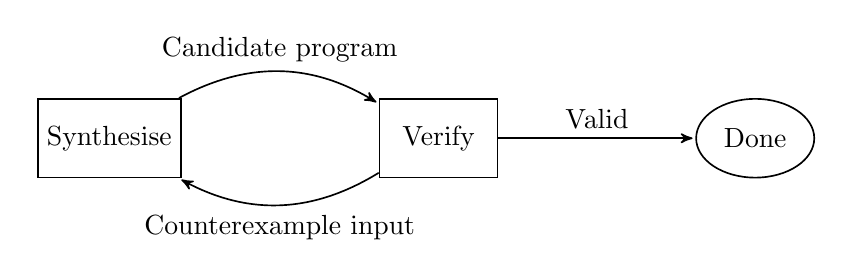
\begin{tikzpicture}[->,>=stealth',shorten >=1pt,auto,
 semithick, initial text=]

  \matrix[nodes={draw, fill=none, shape=rectangle, minimum height=1cm, minimum width=1.5cm},
          row sep=2cm, column sep=2.5cm, ampersand replacement=\&] {
   \node (synth) {Synthesise};
   \&
   \node (verif) {Verify}; %\\
   %\node[draw=none] {};
   \&
   \node[ellipse] (done) {Done}; \\
  };

   \path
    (synth) edge [bend left] node {Candidate program} (verif)
    (verif) edge [bend left] node {Counterexample input} (synth)
    (verif) edge node {Valid} (done);
 \end{tikzpicture}
 }
 \end{center}
 
 \caption{Abstract synthesis refinement loop
 \label{fig:abstract-refinement}}
\end{figure}



\begin{figure}
{\small
\begin{center}
\setlength{\tabcolsep}{16pt}
Integer arithmetic instructions:

\begin{tabular}{llll}
 \verb|add a b| & \verb|sub a b| & \verb|mul a b| & \verb|div a b| \\
 \verb|neg a| &   \verb|mod a b| & \verb|min a b| & \verb|max a b|
\end{tabular}

\medskip

Bitwise logical and shift instructions:

\begin{tabular}{lll}
 \verb|and  a b| & \verb|or   a b| & \verb|xor a b| \\
 \verb|lshr a b| & \verb|ashr a b| & \verb|not a|
\end{tabular}

\medskip

Unsigned and signed comparison instructions:

\begin{tabular}{lll}
 \verb|le  a b| & \verb|lt  a b| & \verb|sle  a b| \\
 \verb|slt a b| & \verb|eq  a b| & \verb|neq  a b|
\end{tabular}

Miscellaneous logical instructions:

\begin{tabular}{lll}
 \verb|implies a b| & \verb|ite a b c| & 
\end{tabular}

Floating-point arithmetic:

\begin{tabular}{llll}
 \verb|fadd a b| & \verb|fsub a b| & \verb|fmul a b| & \verb|fdiv a b| 
\end{tabular}


\end{center}
}
 \caption{The language $\mathcal{L}$}
 \label{fig:l-language}
\end{figure}

\subsection{The Synthesis Algorithm}

We use Counterexample Guided Inductive Synthesis
(CEGIS)~\cite{lezama-thesis,sketch, DBLP:conf/iclp/BrainCVF06} to find an
$\mathcal{L}$-program satisfying our specification.  The core of the CEGIS
algorithm is the refinement loop shown in Fig.~\ref{fig:abstract-refinement}
and detailed in Algorithm~\ref{alg:cegis}.  The algorithm is divided into
two procedures: {\sc synth} (see Figure~\ref{fig:synth-dfd}) and {\sc
verif}, which interact via a finite set of test vectors {\sc inputs}.

The {\sc synth} procedure tries to find existential witnesses $(P, x_0)$
that satisfy the partial specification:
%
\[
 \exists P, x_0 . \forall x \in \text{\sc inputs} . \sigma(P, x_0, x)
\]

If {\sc synth} succeeds in finding a witness $(P, x_0)$, this witness is a
candidate solution to the full synthesis formula.  We pass this candidate
solution to {\sc verif} which determines whether it does satisfy
the specification on all inputs by checking satisfiability of the
verification formula:
%
\[
 \exists x . \lnot \sigma(P, x_0, x)
\]

If this formula is unsatisfiable, the candidate solution is in fact a
solution to the synthesis formula and so the algorithm terminates. 
Otherwise, the witness $x$ is an input on which the candidate solution fails
to meet the specification.  This witness $x$ is added to the {\sc inputs}
set and the loop iterates again.

Concretely, {\sc synth} is implemented as shown in
Figure~\ref{fig:synth-dfd}.  We start by taking the termination
specification and generating a \newC program which takes as input a candidate
$(P, x_0)$ and asserts that the candidate fails to meet the specification on
at least one of the elements of {\sc inputs}.  So this program is unsafe iff
there is some candidate $(P, x_0)$ satisfying the specification for all the
elements of {\sc inputs}.  Finding a new candidate solution is therefore
reduced to model checking this \newC program, which by construction is loop
free.  The model checking is done using a combination of symbolic Bounded Model
Checking (BMC), explicit state enumeration and genetic programming (GP) running in
parallel.
Finally, if any of the model checkers finds a candidate solution, it returns it
and the others are killed.  The form of
this candidate solution is yet another program, this time written in the
proof language $\mathcal{L}$.

As well as efficiency, compiling the original source code of the program
under analysis has the advantage of guaranteeing that we are verifying the
exact semantics of the program as understood by a compiler, rather than some
ad-hoc abstraction of its semantics.

Similarly to {\sc synth}, the {\sc verif} procedure is implemented by
creating a \newC program that is unsafe iff some input exists on which the
candidate solution fails to meet the specification.  Again, symbolic and
explicit-state model checking are used to decide the satisfiability of the
verification formula\footnote{GP is not used, since it is inherently incomplete.}.


\begin{figure*}
\begin{center}
\tikzstyle{file}=[draw, text width=7.0em, text centered,
  minimum height=1.5em]
\tikzstyle{process} = [draw, minimum height=3em, circle]
\tikzstyle{line} = [draw, color=black, -latex']

\def\Divide#1#2{%
 \coordinate(a) at ($(#1.east) !.5! (#2.west)$);
 \coordinate(b) at (a |- 0,-3);
 \draw[dotted] (b) -- ++(0, 4.5);
}

%\resizebox{\linewidth}{!}{
\begin{tikzpicture}[font=\sffamily]

\node [file] (pua) {input.c};

\path (pua.east)+(2,0) node [file] (spec) {\sc Termination Specification};
\path (spec.south)+(0.0, -1) node [file] (inputs) {\sc Tracked Inputs};
%% \path (synth.south)+(0.0, -0.5) node [file] (tests) {\sc tests.c};
%% \path (tests.south)+(0.0, -0.5) node [file] (interpreter) {\sc interpreter.c};
%% \path (interpreter.south)+(0.0, -0.5) node [file] (spec) {\sc spec.c};

%% \path (spec.east)+(2.0, -0.25) node [process] (merged) {merge};
\path (spec.east)+(2.0, -0.75) node [file] (file) {synth.c};

\path (file.east)+(2.0, 1.5) node [process] (cbmc) {\sc cbmc};
\path (file.east)+(2.0, 0.0) node [process] (gcc) {\sc Search};
\path (file.east)+(2.0, -1.5) node [process] (gp) {\sc GP};

\path (gcc.east)+(2.5, 0.0) node [file] (out) {Candidate Proof};

%\path [line] (spec) -- (merged);

\path [line] (pua) -- (spec);

\path [line] (spec) -- (file);
\path [line] (inputs) -- (file);

\path [line] (file) -- (cbmc);
\path [line] (file) -- (gcc);
\path [line] (file) -- (gp);


\path [line] (cbmc) -- (out);
\path [line] (gcc) -- (out);
\path [line] (gp) -- (out);

\Divide{pua}{spec}{puaspec}
%\Divide{spec}{file}{specfile}
\Divide{file}{gcc}{filegcc}
\Divide{gcc}{out}{gccout}

\draw (pua |- 0,-3) node [align=center] {Input program \\ (written in C)};

\coordinate (midspec) at ($(spec) !.5! (file)$);
\draw (midspec |- 0,-3) node [align=center] {Automatically generated specification \\ (written in C)};
%\draw (file |- 0,-3) node {Spec};
\draw (gcc |- 0,-3) node [align=center] {Model checker};
\draw (out |- 0,-3) node [align=center] {Proof \\ (written in $\mathcal{L}$)};

\end{tikzpicture}
%}
\end{center}

\caption{Schematic diagram of {\sc synth}}
\label{fig:synth-dfd}
\end{figure*}



\subsection{Candidate Generation Strategies}
\noindent{\bf Explicit Proof Search.} The simplest strategy for finding candidates
is to just exhaustively enumerate them all, starting with the shortest and
progressively increasing the number of instructions.  This strategy
is implemented by the {\sc ExplicitSearch} routine.  Since the set of
$\mathcal{L}$-programs is recursively enumerable, this procedure is complete.
\\

\noindent{\bf Symbolic Bounded Model Checking.} Another complete method for generating
candidates is to simply use BMC on the {\sc synth.c} program.  As with explicit
search, we must progressively increase the length of the $\mathcal{L}$-program we search for
in order to get a complete search procedure.
\\

\noindent {\bf Genetic Programming and Incremental Evolution.} \label{sec:gp}
Our final strategy is genetic programming
(GP)~\cite{langdon:fogp,brameier2007linear}.  GP provides an adaptive way of
searching through the space of $\mathcal{L}$-programs for an individual
that is ``fit'' in some sense.  We measure the
fitness of an individual by counting the number of tests in {\sc inputs}
for which it satisfies the specification.

To bootstrap GP in the first iteration of the CEGIS loop, we generate a population
of random $\mathcal{L}$-programs. We then iteratively evolve this population by
applying the genetic operators {\sc crossover} and {\sc mutate}.
{\sc Crossover} combines selected existing programs into new programs,
whereas {\sc mutate} randomly changes parts of a single program.
Fitter programs are more likely to be selected.


% The {\sc crossover} operator takes two programs and combines their
% code in some way to create a new program.  Programs are selected to be
% {\sc crossover}ed according to their fitness -- fitter programs are more
% likely to be selected to become parents.

% The {\sc mutate} operator takes a single program and randomly changes parts
% of its code, again creating a new program.

Rather than generating a random population at the beginning of each subsequent
iteration of the CEGIS loop, we start with the population we had at the end of the
previous iteration.  The intuition here is that this population contained
many individuals that performed well on the $k$ inputs we had before, so
they will probably continue to perform well on the $k+1$ inputs we have now.
In the parlance of evolutionary programming, this is known as
incremental evolution~\cite{Gomez97incrementalevolution}.

% In the setting of program synthesis, genetic programming can be very
% usefully combined with the concept of incremental evolution.  The idea is
% that in order to evolve a program that is adequate for some difficult task,
% it is often helpful to first evolve a population that as an ensemble is good
% at some simpler variation of the task.  This principle leads us to the
% observation that each round of the CEGIS loop can be thought of as creating
% a more difficult problem for the GP synthesiser to solve.  Therefore, if GP
% finds a candidate program which is correct for the $k$ inputs so far
% observed, but is not correct for the full specification, that candidate
% program came from a population that was ``good'' for the specification
% restrict to those $k$ inputs.  The next time round the CEGIS loop, the
% problem GP must solve is slightly harder -- any solution to this new problem
% must be correct for the previous $k$ inputs and also whatever new input was
% added by the previous iteration of {\sc verif}.  It therefore makes sense to
% begin the $k+1$st round of evolution with the population at the end of the
% $k$-th round.


\section{Soundness, Completeness and Complexity}

Termination for bit-vector programs is known to be
PSPACE-complete~\cite{DBLP:conf/tacas/CookKRW10}.  We first record the
expected results for soundness and completeness of our algorithm for
deciding it.  Our strategy for proving soundness and completeness
is first to prove that Algorithm~\ref{alg:cegis} (as instanciated
with \newC as a background logic) is a semi-decision
procedure.  Next, we will show that $\mathcal{L}$ is expressive enough
to compute (non-)termination proofs for every bit-vector program.
We will then combine these results to show that the procedure as a whole
terminates with a valid proof for every input program.
%
\begin{theorem}\label{thm:synth-sound}
Algorithm~\ref{alg:cegis} is sound -- if it terminates with witness $(P, x_0)$, then
$(P, x_0) \models \sigma$.
\end{theorem}

\begin{proof}
 The procedure {\sc Synthesise} terminates only if {\sc Verif} returns ``valid''.  In that
 case, $\exists x . \lnot \sigma(P, x_0, x)$ is unsatisfiable and so $\forall x . \sigma(P, x_0, x)$ holds.
\end{proof}

\begin{theorem}
 \label{thm:synth-semicomplete}
 If the existential first-order theory used to express the specification $\sigma$ is decidable
 and the domain of inputs $X$ is finite,
 Algorithm~\ref{alg:cegis} is semi-complete -- if a solution $(P, x_0) \models \sigma$
 exists then Algorithm~\ref{alg:cegis} will terminate.  However, if no program
 satisfies the specification, the algorithm may not terminate.
\end{theorem}

\begin{proof}
 If the domain $X$ is finite then the loop in procedure {\sc Synthesise} can only
 iterate $\| X \|$ times, since by this time all of the elements of $X$ would have been
 added to the inputs set.  Therefore if the {\sc Synth} procedure always terminates,
 Algorithm~\ref{alg:cegis}.

 Since the {\sc ExplicitSearch} routine enumerates all programs (as can be seen by induction on
 the program length $l$), it will eventually enumerate a program that meets the specification
 in whatever set of inputs are currently being tracked, since by assumption such a program
 exists.  Since the first-order theory is
 decidable, the query in {\sc Verif} will succeed for this program, causing the algorithm to terminate.
 The set of correct programs is therefore recursively enumerable and Algorithm~\ref{alg:cegis}
 enumerates this set, so it is semi-complete.
\end{proof}

\begin{corollary}
\label{cor:cegis-newc}
 Since safety of \newC programs is decidable, Algorithm~\ref{alg:cegis} is semi-complete
 when instanciated with \newC as a background theory.
\end{corollary}


% \begin{theorem}
% \label{thm:sound}
%  {\sc Headshot} is sound -- if it returns a verdict of termination, the program under
%  analysis terminates on all inputs.  Similarly if it returns a verdict of non-termination,
%  the program under analysis has at least one infinite execution.
% \end{theorem}
% 
% \begin{proof}
%  This is a direct consequence of Theorems~\ref{thm:ut}, \ref{thm:ct}, \ref{thm:ont}, \ref{thm:cnt} and \ref{thm:synth-sound}.
% \end{proof}

We will now show that $\mathcal{L}$ is expressive enough to encode (non-)termination proofs for
every bit-vector program.

\begin{lemma}
 \label{lem:l-func}
 Every function $f: X \to Y$ for finite $X$ and $Y$ is computable by a finite $\mathcal{L}$-program.
\end{lemma}

\begin{proof}
Without loss of generality, let $X = Y = \mathbb{N}_b^k$ the set of
$k$-tuples of natural numbers less than $b$.
A very inefficient construction which computes the first coordinate
of the output $y$ is:
%
\begin{verbatim}
t1 = f(0)
t2 = v1 == 1
t3 = ITE(t2, f(1), t1)
t4 = v1 == 2
t5 = ITE(t4, f(2), t3)
...
\end{verbatim}
%
Where the \verb|f(n)| are literal constants that are to appear in the program text.
This program is of length $2b - 1$, and so all $k$ co-ordinates of the output $y$
are computed by a program of size at most $2bk - k$.
\end{proof}

\begin{corollary}
 Every finite subset $A \subseteq B$ is computable by a finite $\mathcal{L}$-program
 by setting $X = B, Y = 2$ in Lemma~\ref{lem:l-func}.
\end{corollary}


\begin{theorem}
\label{thm:l-term}
 Every terminating bit-vector program has a ranking function that is expressible in $\mathcal{L}$.
\end{theorem}

\begin{proof}
%
Let $v_1, \ldots, v_k$ be the variables of the program $P$ under analysis,
and let each be $b$ bits wide.  Its state space $\mathcal{S}$ is then of
size $2^{bk}$.  A~ranking function $R: \mathcal{S} \to \mathcal{D}$ for $P$
exists iff $P$ terminates.  Since $R$ is injective, we have that $\|
\mathcal{D} \| \geq \| \mathcal{S} \|$.  If $\| \mathcal{D} \| > \|
\mathcal{S} \|$, we can construct a function $R': \mathcal{S} \to
\mathcal{D'}$ with $ \| \mathcal{D'} = \| \mathcal{S} \|$ by just setting
$R' = R|_\mathcal{S}$, i.e.~$R'$ is just the restriction of $R$ to
$\mathcal{S}$.  Since $\mathcal{S}$ already comes equipped with a natural
well ordering we can also construct $R'' = \iota \circ R'$ where $\iota:
\mathcal{D'} \to \mathcal{S}$ is the unique order isomorphism from
$\mathcal{D'}$ to $\mathcal{S}$.  So assuming that $P$ terminates, there is
some ranking function $R''$ that is just a permutation of $\mathcal{S}$.  If
the number of variables $k > 1$ then in general the ranking function will be
lexicographic with dimension $\leq k$ and each co-ordinate of the output
being a single $b$-bit value.

Then by Lemma~\ref{lem:l-func} with $X = Y = \mathcal{S}$, there exists
a finite $\mathcal{L}$-program computing $R''$.

% Since {\sc Kalashnikov} enumerates all programs in order of
% length, it will eventually check a program computing each permutation of
% $\mathcal{S}$ and so will eventually check a program computing the ranking
% function $R''$.  Checking that a single program satisfies the specification
% is a decidable problem, and the search as a whole terminates.
%
\end{proof}

\begin{theorem}
\label{thm:l-nonterm}
 Every non-terminating bit-vector program has a non-termination proof expressible in $\mathcal{L}$.
\end{theorem}

\begin{proof}
 A non-termination proof is a triple $\langle N, C, x_0 \rangle$ where $N \subseteq \mathcal{S}$ is
 a (finite) recurrence set and $C : \mathcal{S} \to \mathcal{S}$ is a Skolem function choosing
 a successor for each $x \in N$.  Since $\mathcal{S}$ is finite, so by Lemma~\ref{lem:l-func} both
 $N$ and $C$ are computed by finite $\mathcal{L}$-programs.
\end{proof}

\begin{theorem}
 \label{thm:generalised-sat}
 The generalised termination formula for loop $L$ (Definiton~\ref{def:general-termination}) is satisfiable
 when $P_N$ and $P_T$ range over \mbox{$\mathcal{L}$-computable} functions.
\end{theorem}

\begin{proof}
 For any $P, P', \sigma, \sigma$, if $P \models \sigma$ then $(P, P') \models \sigma \vee \sigma'$.

 By Theorem~\ref{thm:l-term}, if $L$ terminates then there exists a termination proof $P_T$ expressible
 in $\mathcal{L}$.  Since $\phi$ is an instance of {\bf [CT]}, $P_T \models \phi$ (Theorem~\ref{thm:ct}) and
 for any $P_N$, $(P_T, P_N) \models \phi \vee \psi$.

 Similarly if $L$ does not terminate for some input, by Theorem~\ref{thm:l-nonterm} there is a non-termination
 proof $P_N$ expressible in $\mathcal{L}$.  $\psi$ is an instance of {\bf [SNT]} and so $P_N \models \psi$
 (Theorem~\ref{thm:snt}), hence for any $P_T$, $(P_T, P_N) \models \phi \vee \psi$.

 So in either case ($L$ terminates or does not), there is a witness in $\mathcal{L}$ satisfying
 formula {\bf [GT]}: $\phi \vee \psi$.
\end{proof}

\begin{theorem}
 Algorithm~\ref{alg:termination} is sound and complete -- it terminates for all input loops $L$ with
 a correct termination verdict.
\end{theorem}

\begin{proof}
 By Theorem~\ref{thm:generalised-sat}, the specification \lstinline!spec! is satisfiable.  Corollary~\ref{cor:cegis-newc}
 shows that Algorithm~\ref{alg:cegis} is semi-complete, and so the call to {\sc Synthesise} terminates with a witness $(P_T, P_N)$.
 If $L$ terminates then $P_T$ is a termination proof (Theorem~\ref{thm:ct}).  Otherwise $P_N$ is a non-termination proof
 (Theorem~\ref{thm:snt}).  Exactly one of these cases holds, and the background theory being decidable means that each
 call to \lstinline|decide()| will terminate, which allows us to determine which of $P_T$ and $P_N$ is a correct proof.
\end{proof}

Hence Algorithm~\ref{alg:termination} is sound and complete for bit-vector termination.

Theorem~\ref{thm:synth-semicomplete} provides a time bound -- the CEGIS loop can iterate at most
$2^bk$ times where $k$ is the number of variables used by $L$ and
$b$ is the number of bits used to store each variable.
The $i$th iteration of the loop requires solving 2 NP-complete problems of size $i \times \| L\|$
with $\| L \| $ the size of the program-under-analysis computing $\| L \|$.  So if 
the CEGIS loop iterates $n$ times, the
runtime is bounded by $2 \times n \times NP(n \times \| L \|)$, which is bounded
by $2^{bk + 1} NP(2^{bk} \| L \|)$.  Clearly the runtime is affected most strongly by $n$,
the total number of iterations of the CEGIS loop.

We will now show that our time complexity is asymptotically a function of
the Kolmogorov complexity of the (non-)termination proof, and argue
that this gives our procedure various desirable qualities in practical
appliations.
%
\begin{theorem}
 {\sc Kalashnikov} has time complexity $NP^{NP}(K(\sigma))$.
\end{theorem}

\begin{theorem}
 {\sc Headshot} uses a single call to {\sc Kalashnikov} and uses an encoding with $O(1)$
 overhead.  It therefore has time complexity $NP^{NP}(K(\tau(P))$ where $\tau(P)$ is the
 termination specification for program $P$.
\end{theorem}

In Section~\ref{sec:synthesis} we will describe a procedure for solving the synthesis formula.
This procedure has the property that it will find the shortest program meeting the
specification, and as a consequence the runtime of the program synthesiser is dominated
by the size of this shortest program.  To frame the discussion of the runtime of our
termination proving procedure, we first recall the definition of the Kolmogorov complexity
of a function $f$:

\begin{definition}[Kolmogorov complexity]
 The Kolmogorov complexity $K(f)$ is the length of the shortest program that
 computes~$f$.
\end{definition}

We can extend this definition slightly to talk about the Kolmogorov complexity of a
synthesis problem in terms of its specification:

\begin{definition}[Kolmogorov complexity of a synthesis problem]
 The Kolmogorov complexity of a program specification $K(\sigma)$ is the length of the shortest
 program $P$ such that $P \models \sigma$.
\end{definition}

We will later show that the time complexity of our synthesis procedure is $NP^{NP}(K(\sigma))$,
which means that for even moderately large $K(\sigma)$ our procedure is intractably slow.  Conversely
if $K(\sigma)$ is small we will be able to find a termination proof, regardless of other parameters
such as the size of the program under analysis.  To put this another way, under the assumption
that $K(\sigma)$ is small for a program's termination problem, we will find a ranking function
quite rapidly.  We will now investigate the properties of functions with low Kolmogorov complexity,
and show that the assumption of a low-Kolmogorov ranking function is much weaker than the assumption
of a linear ranking function.


\begin{theorem}
 Linear functions have low Kolmogorov complexity.
\end{theorem}

\begin{proof}
 The function $f: X \to Y$ can be computed with a program consisting of
 $2 \cdot \dim(X) \cdot \dim(Y) - \dim(Y)$ instructions (1 multiplication and 1 addition for
 each cell in the matrix representing $f$).  Therefore,
 $K(f) \leq 2 \cdot \dim(X) \cdot \dim(Y) - \dim(Y)$.
\end{proof}

\begin{theorem}
Assuming a reasonable program encoding, the probability that a random program of length $l$ computes
a linear function is $O(2^{-l})$.
\end{theorem}

\begin{proof}
 (Do this proof properly).
 
 Otherwise, we'd need to have an exponential number of programs computing the same function.
 That would be an unreasonable program encoding.
\end{proof}


Therefore the number of nonlinear functions $f$ with $K(f) \leq \kappa$
grows exponentially with $\kappa$, while the number of linear functions
grows only linearly.  This shows that assuming the existence of a linear
ranking function is much stronger than assuming the existence of a short
termination proof.  In addition to being a much weaker assumption,
we argue that low Kolmogorov complexity is a more natural assumption than
linearity.  Humans tend to write programs they can understand.  It's hard
to quantify exactly what ``understandable'' means, but we think that
``having a short proof'' is closer to the mark than ``having a linear proof''.


\section{Experiments}

To evaluate our algorithm, we implemented two tools: one to generate a
termination specification from a C program, and one to synthesise a proof
from the specification.  We ran the resulting termination prover,
named {\sc Juggernaut}, on 47
benchmarks taken from the literature and SV-COMP'15~\cite{svcomp15}.  To
provide a comparison point, we also ran {\sc ARMC}~\cite{armc-website} on
the same benchmarks.  Each tool was given a time limit of 180s, and was
run on an unloaded 8-core 3.07\,GHz Xeon X5667 with 50\,GB of RAM.  The
results of these experiments are given in Figure~\ref{fig:experiments}.

It should be noted that the comparison here is imperfect, since {\sc ARMC}
is solving a slightly different problem -- it checks whether the program
under analysis would terminate if run with unbounded integer variables,
while we are checking whether the program terminates with fixed-width
integer variables.  This means that {\sc ARMC}'s verdict differs from ours
in 3 cases (due to the differences between integer and bit-vector
semantics).  There are a further 7 cases where our tool is able to find a
proof and {\sc ARMC} cannot, which we believe is due to our more expressive
proof language.  In 3 cases, {\sc ARMC} times out while our tool is able to
find a termination proof.  Of these, 2 cases have nested loops and the
third has an infinite number of terminating lassos.  This is not a problem for us,
but can be difficult for provers that enumerate lassos.

On the other hand, {\sc ARMC} is \emph{much} faster than our tool.  While
this difference can partly be explained by much more engineering time being
invested in {\sc ARMC}, we feel that the difference is probably inherent to
the difference in the two approaches -- our algorithm is complete and
bit-vector accurate, which comes at the cost of efficiency.
{\sc Juggernaut} is slow, but unstoppable in its
termination capabilities if you are willing to wait for it.

The final column in Figure~\ref{fig:experiments} gives the number of
iterations of the CEGIS loop our synthesiser performed.  While the
theoretical bound for the number of CEGIS iterations is very large
(exponential in the amount of space used by the program), these results
demonstrate that in practice the number of iterations required is usually
small.

Of the 47 benchmarks, 2 use nonlinear operations in the program (loop6 and loop11),
and 5 have nested loops (svcomp6, svcomp12, svcomp18, svcomp40, svcomp41).
{\sc Juggernaut} handles the nonlinear cases correctly and rapidly.
It solves 2 of the 5 nested loops in less than 30s, but times out on the other
3.  Of these 3 timeouts, 2 (svcomp40 and svcomp41) are due to program constants that
are too large to be handled with our default settings.  Increasing
our default word width from 3 bits to 5 bits allowed us to prove termination
for both these benchmarks in less than 30s; these results are marked with a *.

In conclusion, while they show that our tool is not yet production ready,
these experiments confirm our conjecture that synthesis can be used
effectively to prove termination and non-termination.  In particular,
for programs with nested loops, nonlinear arithmetic and complex
termination arguments, the versatility of unrestricted synthesis
is very valuable.

\begin{figure}
\centering
\scriptsize
\begin{tabular}{|l|@{}c@{}||@{}c@{}|r||@{}c@{}|r|r|}
\hline
          &             & \multicolumn{2}{|c||}{\sc ARMC} & \multicolumn{3}{|c|}{\sc Juggernaut} \\
Benchmark & \,Expected\, & \,Verdict\, & Time & \,Verdict\, & Time & \#It.\\
    \hline
    \hline
loop1.c & \tick & \tick & 0.06s & \tick & 1.3s & 1\\ 

loop2.c & \tick & \tick & 0.06s & \tick & 1.4s & 4\\ 

loop3.c & \tick & \tick & 0.06s & \tick & 1.8s & 8\\ 

loop4.c & \tick & \tick & 0.12s & \tick & 2.9s & 18\\ 

loop5.c & \tick & \tick & 0.12s & \tick & 5.3s & 18\\ 

loop6.c & \tick & \tick & 0.05s & \tick & 1.2s & 1\\ 

loop7.c & \tick & \xmark & 0.05s & \tick & 8.3s & 17\\ 

loop8.c & \tick & \xmark & 0.06s & \tick & 1.3s & 1\\ 

loop9.c & \tick & \tick & 0.11s & \tick & 1.6s & 1\\ 

loop10.c & \tick & \xmark & 0.05s & \tick & 1.3s & 1\\ 

loop43.c & \tick & \tick & 0.07s & \tick & 1.5s & 1\\ 

loop44.c & \xmark & \xmark & 0.05s & \xmark & 10.5s & 9\\ 

loop45.c & \tick & \tick & 0.12s & \tick & 4.3s & 18\\ 

loop46.c & \tick & \xmark & 0.05s & \tick & 1.5s & 2\\ 

loop47.c & \tick & \tick & 0.10s & \tick & 1.8s & 1\\ 

loop48.c & \tick & \tick & 0.06s & \tick & 1.4s & 4\\ 

loop49.c & \xmark & \xmark & 0.05s & ? & T/O & 206\\ 

svcomp1.c & \tick & \tick & 0.11s & \tick & 2.3s & 2\\ 

svcomp2.c & \tick & \tick & 0.05s & \tick & 1.5s & 9\\ 

svcomp3.c & \tick & \tick & 0.15s & \tick & 146.4s & 43\\ 

svcomp4.c & \xmark & \xmark & 0.09s & \xmark & 2.1s & 7\\ 

svcomp5.c & ? & \tick & 0.38s & ? & T/O & 46\\ 

svcomp6.c & \tick & ? & T/O & \tick & 29.1s & 28\\ 

svcomp7.c & \tick & \tick & 0.09s & \tick & 5.5s & 17\\ 

svcomp8.c & ? & \xmark & 0.05s & ? & T/O & 37\\ 

svcomp9.c & \tick & \tick & 0.10s & \tick & 1.5s & 8\\ 

svcomp10.c & \tick & \tick & 0.11s & \tick & 4.5s & 18\\ 

svcomp11.c & \tick & \tick & 0.20s & \tick & 14.6s & 33\\ 

svcomp12.c & \tick & ? & T/O & \tick & 10.9s & 24\\ 

svcomp13.c & ? & \xmark & 0.07s & \tick & 35.1s & 62\\ 

svcomp14.c & \tick & ? & T/O & \tick & 30.8s & 26\\ 

svcomp15.c & ? & \xmark & 0.12s & ? & T/O & 191\\ 

svcomp16.c & \tick & \tick & 0.06s & \tick & 2.2s & 3\\ 

svcomp17.c & \tick & \tick & 0.05s & ? & T/O & 32\\ 

svcomp18.c & ? & \xmark & 0.27s & ? & T/O & 26\\ 







svcomp25.c & ? & \xmark & 0.05s & ? & T/O & 26\\ 

svcomp26.c & \tick & \tick & 0.26s & \tick & 3.2s & 23\\ 

svcomp27.c & \xmark & \tick & 0.11s & ? & T/O & 67\\ 

svcomp28.c & ? & \tick & 0.13s & ? & T/O & 79\\ 

svcomp29.c & ? & \xmark & 0.05s & ? & T/O & 1\\ 








svcomp37.c & \tick & \tick & 0.16s & \tick & 2.1s & 10\\ 

svcomp38.c & \tick & \tick & 0.10s & ? & T/O & 1\\ 

svcomp39.c & ? & \tick & 0.25s & ? & T/O & 1\\ 

svcomp40.c & ? & \xmark & 0.07s & ? & T/O & 30\\ 

svcomp41.c & ? & \xmark & 0.07s & ? & T/O & 27\\ 

svcomp42.c & ? & \tick & 0.22s & ? & T/O & 85\\ 


    \hline
\end{tabular}

Key: \tick = terminating, \xmark = non-terminating, ? = unknown (tool terminated with an inconclusive verdict).

Times marked with a * were run with non-default command line flags.

\caption{Experimental results\label{fig:experiments}}
 \end{figure}

\section{Conclusions and Related Work}

There has been substantial prior work on automated program termination
analysis.  Figure~\ref{fig:handletable} summarises the related work with
respect to the assumptions they make about programs and ranking functions. 
Most of the techniques are specialised in the synthesis of linear ranking
functions for linear programs over integers (or
rationals)~\cite{DBLP:conf/pldi/CookPR06, DBLP:conf/cav/LeeWY12,
DBLP:conf/popl/Ben-AmramG13, DBLP:conf/vmcai/P04,
DBLP:conf/atva/HeizmannHLP13, DBLP:conf/cav/BradleyMS05,
DBLP:conf/tacas/CookSZ13, DBLP:conf/cav/KroeningSTW10}.  Among them, Lee et
al.~make use of transition predicate abstraction, algorithmic learning, and
decision procedures~\cite{DBLP:conf/cav/LeeWY12}, Leike and Heizmann propose
linear ranking templates~\cite{DBLP:conf/tacas/LeikeH14}, whereas Bradley et
al.~compute lexicographic linear ranking functions supported by inductive
linear invariants~\cite{DBLP:conf/cav/BradleyMS05}.

While the synthesis of termination arguments for linear programs over
integers is indeed well covered in the literature, there is very limited
work for programs over machine integers.  Cook et al.~present a method
based on a reduction to Presburger arithmetic, and a template-matching
approach for predefined classes of ranking functions based on reduction to
SAT- and QBF-solving~\cite{DBLP:conf/tacas/CookKRW10}.  Similarly, the only
work we are aware of that can compute nonlinear ranking functions for
imperative loops with polynomial guards and polynomial assignments
is~\cite{DBLP:conf/vmcai/BradleyMS05}.  However, this work extends only to
polynomials.

Given the lack of research on termination of nonlinear programs, as well as
programs over bit vectors and floats, our work focused on covering these
areas.  One of the obvious conclusions that can be reached from
Figure~\ref{fig:handletable} is that most methods tend to specialise on a
certain aspect of termination proving that they can solve efficiently. 
Conversely to this view, we aim for generality, as we do not restrict the
form of the synthesised ranking functions, nor the form of the input
programs. 

%As a general approach to proving liveness properties, Biere et al.
%propose a translation of liveness checking problems into safety checking problems
%that is however best suited for finding shallow termination arguments 
%\cite{DBLP:journals/entcs/BiereAS02}. 


As mentioned in Section~\ref{sec:intro}, approaches based on Ramsey's
theorem compute a set of local termination conditions that decrease as
execution proceeds through the loop and require expensive reachability
analyses~\cite{DBLP:conf/lpe/CodishG03, DBLP:conf/lics/PodelskiR04,
DBLP:conf/pldi/CookPR06}.  In an attempt to reduce the complexity of
checking the validity of the termination argument, Cook et al.~present an
iterative termination proving procedure that searches for lexicographic
termination arguments~\cite{DBLP:conf/tacas/CookSZ13}, whereas Kroening et
al.~strengthen the termination argument such that it becomes a transitive
relation~\cite{DBLP:conf/cav/KroeningSTW10}. Following the same trend, 
we search for lexicographic nonlinear termination arguments that can be verified 
with a single call to a SAT solver. 


Proving program termination implies the simultaneous search for a
termination argument and a supporting invariant.  Brock\-schmidt et
al.~share the same representation of the state of the termination proof
between the safety prover and the ranking function synthesis
tool~\cite{DBLP:conf/cav/BrockschmidtCF13}.  Bradley et al.~combine the
generation of ranking functions with the generation of invariants to form a
single constraint solving problem such that the necessary supporting
invariants for the ranking function are discovered on
demand~\cite{DBLP:conf/cav/BradleyMS05}.  In our setting, both the ranking
function and the supporting invariant are iteratively constructed in the
same refinement loop.

While program termination has been extensively studied, much less research
has been conducted in the area of proving non-termination.  Gupta et
al.~dynamically enumerate lasso-shaped candidate paths for counterexamples,
and then statically prove their
feasibility~\cite{DBLP:conf/popl/GuptaHMRX08}.  Chen et al.~prove
nontermination via reduction to safety
proving~\cite{DBLP:conf/tacas/ChenCFNO14}.  Their iterative algorithm uses
counterexamples to a fixed safety property to refine an under-approximation
of a program.  In order to prove both termination and non-termination,
Harris et al.~compose several program analyses (termination provers for
multi-path loops, non-termination provers for cycles, and global safety
provers)~\cite{DBLP:conf/sas/HarrisLNR10}.  We propose a uniform treatment
of termination and non-termination by formulating a generalised second order
formula whose solution is a proof of one of them.

\bibliographystyle{abbrvnat}
\bibliography{synth}{}

\end{document}
